



Mathematics is done by writing down statements and proving them. In this course we take that activity itself as our object of study: we write down what a `statement' is as a finite string of symbols, we write down what a `proof' is as a finite list of such strings obeying some rules, and then we prove theorems about the resulting system. The most striking of these -- the completeness theorem -- says that the two ways we have of saying that something follows from something else, the semantic one (`it is true in every situation where the hypotheses hold') and the syntactic one (`there is a proof of it'), give exactly the same answer.

Alongside this we develop set theory, which serves as the arena in which all of the above takes place. We will meet the ordinals, which extend counting past infinity and which give us induction and recursion of unlimited length; Zorn's lemma, which is the form in which the axiom of choice is usually applied; and finally the axioms of Zermelo--Fraenkel set theory, together with a picture of the universe of sets that they describe. The two halves of the course meet at the very end, when we use a set-theoretic construction to write down a sentence of arithmetic that is true but unprovable.

This article constitutes my notes for the `Logic and Set Theory' course, held in Lent 2023 at Cambridge. These notes are \emph{not a transcription of the lectures}, and differ significantly in quite a few areas. Still, all lectured material should be covered.



\section{Propositional Logic}

We begin our study of logic by looking at \emph{propositional logic}, which is the logic of statements built up out of atomic statements using connectives like `and', `or' and `implies'. It is a small enough system that we can prove everything we would want to about it, and it will act as a template for the more elaborate predicate logic that we meet in Section~\ref{sec:predicate}.

\subsection{Languages}

The first thing to do is to say precisely what a statement \emph{is}. It will be a finite string of symbols, built up according to some grammar from a supply of atoms.

\begin{definition}[Language]
  Let $P$ be a set of \vocab{primitive propositions}. Unless otherwise stated we take $P = \{p_1, p_2, \dots\}$. The \vocab{language} $L$, or $L(P)$, is defined inductively by
  \begin{enumerate}[label=(\roman*)]
    \item If $p \in P$, then $p \in L$;
    \item $\bot \in L$ (where we read $\bot$ as `false');
    \item If $p, q \in L$ then $(p \Rightarrow q) \in L$.
  \end{enumerate}
\end{definition}

Every \vocab{proposition} (that is, member of $L$) is a finite string of symbols from the alphabet $\{(, ), \Rightarrow, \bot, p_1, p_2, \dots\}$, satisfying some grammar. It is worth being clear about what the words `defined inductively' mean above, since we will use the same device repeatedly.

We let $L_1 = P \cup \{\bot\}$, and define $L_{n + 1} = L_n \cup \{(p \Rightarrow q) \mid p, q \in L_n\}$. Then $L = \bigcup_{n = 1}^{\infty} L_n$. The rules building up the language are injective and have disjoint ranges, and so there is exactly \emph{one} way in which any element of the language can be constructed from the rules above -- a fact we will lean on constantly, since it is what lets us define things on $L$ by recursion.

This unique readability is best seen by drawing a proposition as a tree, with the primitives and $\bot$ at the leaves and each internal node an application of $\Rightarrow$.

\begin{center}
  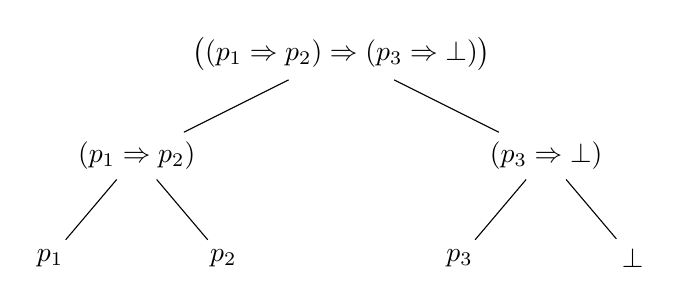
\begin{tikzpicture}[scale=1]
    \node (root) at (0, 2.6) {$\bigl((p_1 \Rightarrow p_2) \Rightarrow (p_3 \Rightarrow \bot)\bigr)$};
    \node (l) at (-2.6, 1.3) {$(p_1 \Rightarrow p_2)$};
    \node (r) at (2.6, 1.3) {$(p_3 \Rightarrow \bot)$};
    \node (l1) at (-3.7, 0) {$p_1$};
    \node (l2) at (-1.5, 0) {$p_2$};
    \node (r1) at (1.5, 0) {$p_3$};
    \node (r2) at (3.7, 0) {$\bot$};
    \draw (root) -- (l); \draw (root) -- (r);
    \draw (l) -- (l1); \draw (l) -- (l2);
    \draw (r) -- (r1); \draw (r) -- (r2);
  \end{tikzpicture}
\end{center}

The proposition drawn above is $\lnot p_3$ implied by $p_1 \Rightarrow p_2$, once we introduce the standard abbreviations $\lnot$ (not), $\land$ (and) and $\lor$ (or), defined by
$$
\lnot p = (p \Rightarrow \bot); \quad p \land q = \lnot(p \Rightarrow \lnot q); \quad p \lor q = (\lnot p) \Rightarrow q.
$$
These are abbreviations only -- our language really does have just the two constructors $\bot$ and $\Rightarrow$. This is purely for convenience: every proof below would go through with more connectives, at the cost of more cases.

\subsection{Semantic Implication}

We now assign `true' or `false' values to propositions. Since a proposition is just a string of symbols, this has to be done by hand.

\begin{definition}[Valuation]
  A \vocab{valuation} is a function $v : L \rightarrow \{0, 1\}$ (where we think of $0$ as false and $1$ as true) such that
  \begin{enumerate}[label=(\roman*)]
    \item $v(\bot) = 0$;
    \item $v(p \Rightarrow q) = 0$ if $v(p) = 1$ and $v(q) = 0$, and $1$ otherwise.
  \end{enumerate}
\end{definition}

One would imagine that it is enough to know how a valuation acts on the primitives, since they are what our language is built out of -- in the same way that a linear map is pinned down by its action on a basis. This is indeed the case.

\begin{proposition}[Valuations are Determined on the Primitives]~
  \begin{enumerate}[label=(\roman*)]
    \item Let $v, v' : L \rightarrow \{0, 1\}$ be valuations that agree on the primitives $p_i$. Then $v = v'$.
    \item Any function $w: P \rightarrow \{0, 1\}$ extends to a valuation.
  \end{enumerate}
\end{proposition}
\begin{proof}
  (i) Clearly $v, v'$ agree on $L_1$. Then if they agree on $p$ and $q$, they agree on $(p \Rightarrow q)$. So by induction they agree on $L_n$ for all $n$, and hence on $L$.

  (ii) Let $v(p) = w(p)$ for all $p \in P$ and $v(\bot) = 0$, to obtain $v$ on the set $L_1$. Assuming $v$ is defined on $p, q$ we can define it at $(p\Rightarrow q)$ in the obvious way. Since each element of $L$ is built up in exactly one way, this consistently defines $v$ on all of $L$.
\end{proof}

In other words, valuations on $L$ correspond exactly to functions $P \to \{0,1\}$, which is what makes truth tables work.

\begin{definition}[Tautology]
  A \vocab{tautology} is an element $t \in L$ such that $v(t) = 1$ for every valuation $v$. We write $\models t$.
\end{definition}

\begin{example}[Some Tautologies]
  Each of the following is a tautology, as one checks by running through the (at most eight) possibilities for the values of the primitives involved.
  \begin{enumerate}[label=(\roman*)]
    \item $p \Rightarrow (q \Rightarrow p)$. If $v(p) = 0$ then the whole thing is $1$ immediately, and if $v(p) = 1$ then $v(q \Rightarrow p) = 1$.
    \item $\lnot \lnot p \Rightarrow p$, that is, $((p \Rightarrow \bot) \Rightarrow \bot) \Rightarrow p$. If $v(p) = 1$ this is $1$, and if $v(p) = 0$ then $v(p \Rightarrow \bot) = 1$ so $v(\lnot \lnot p) = 0$.
    \item $[p \Rightarrow (q \Rightarrow r)] \Rightarrow [(p \Rightarrow q) \Rightarrow (p \Rightarrow r)]$. The only way for this to fail is $v(p) = v(q) = 1$ and $v(r) = 0$, and then the antecedent is already $0$.
  \end{enumerate}
  On the other hand $p \Rightarrow q$ is not a tautology, since we may take $v(p) = 1$ and $v(q) = 0$.
\end{example}

In practice one checks a tautology by drawing a truth table, listing the values of the primitives down the side and computing the value of each subformula.

\begin{example}[A Truth Table]
  We verify that $(\lnot p \Rightarrow \lnot q) \Rightarrow (q \Rightarrow p)$ is a tautology. Writing $v(p)$ and $v(q)$ in the first two columns:
  \begin{center}
    \begin{tabular}{cc|cc|cc}
      $v(p)$ & $v(q)$ & $v(\lnot p)$ & $v(\lnot q)$ & $v(\lnot p \Rightarrow \lnot q)$ & $v(q \Rightarrow p)$ \\ \hline
      $0$ & $0$ & $1$ & $1$ & $1$ & $1$ \\
      $0$ & $1$ & $1$ & $0$ & $0$ & $0$ \\
      $1$ & $0$ & $0$ & $1$ & $1$ & $1$ \\
      $1$ & $1$ & $0$ & $0$ & $1$ & $1$ \\
    \end{tabular}
  \end{center}
  In every row the last two columns agree, so the implication between them takes the value $1$ throughout.
\end{example}

\begin{remark}
  Since a valuation is determined by its values on the primitives, a formula in $n$ primitives determines a function $\{0,1\}^n \to \{0,1\}$. Conversely every such function arises from a formula: one may write down a disjunction of conjunctions, one for each row of the truth table taking the value $1$. So our two connectives $\bot$ and $\Rightarrow$ are already \emph{adequate}, in the sense that every truth function is expressible.
\end{remark}

Usually we are not interested in statements that hold outright, but in statements that hold given some hypotheses.

\begin{definition}[Semantic Implication]
  Let $S \subseteq L$ and $t \in L$. We say $S$ \vocab{entails} or \vocab{semantically implies} $t$, written $S \models t$, if $v(t) = 1$ whenever $v(s) = 1$ for all $s \in S$.
\end{definition}

\begin{definition}[Model]
  We say that $v$ is a \vocab{model} of $S$ in $L$ if $v(s) = 1$ for all $s \in S$.
\end{definition}

So the statement $S \models t$ is precisely the statement that every model of $S$ is also a model of $t$, and the notation $\models t$ is consistent with what we had before, being the same as $\emptyset \models t$.

\begin{example}
  We have $\{p \lor q, \lnot p\} \models q$: if $v(\lnot p) = 1$ then $v(p) = 0$, and $p \lor q$ abbreviates $\lnot p \Rightarrow q$, so $v(q) = 1$. On the other hand $\{p \Rightarrow q\} \not\models p$, as witnessed by the valuation sending every primitive to $0$.
\end{example}

\subsection{Syntactic Implication}

Semantic implication asks us to check every valuation, of which there are infinitely many. What we do in practice instead is give a \emph{proof}. To make that notion precise we need a system of axioms and deduction rules.

\begin{axiom}[Axiom Scheme for Propositional Logic]~
  \begin{enumerate}[label=(\arabic*)]
    \item $p \Rightarrow (q \Rightarrow p)$ for all $p, q \in L$;
    \item $[p \Rightarrow (q \Rightarrow r)] \Rightarrow [(p \Rightarrow q) \Rightarrow (p \Rightarrow r)]$ for all $p, q, r \in L$;
    \item $(\lnot \lnot p) \Rightarrow p$ for all $p \in L$.
  \end{enumerate}
\end{axiom}

Each of these is really an axiom \emph{scheme}, since each line above is a whole set of axioms, one for each choice of the propositions involved. Notice also that each of them is a tautology -- as one would hope, and as we will need for soundness.

For our deduction rules we take only \vocab{modus ponens}: from $p$ and $p \Rightarrow q$ we may deduce $q$.

\begin{definition}[Syntactic Implication]
  For $S \subseteq L$ and $t \in L$, we say $S$ \vocab{proves} or \vocab{syntactically implies} $t$, written $S \vdash t$, if there is a finite sequence $t_1, \dots, t_n = t$ of elements of $L$ such that each $t_i$ is either an axiom, or a member of $S$, or is obtained as $q$ where $t_j = p$ and $t_k = (p \Rightarrow q)$ for some $j, k < i$.

  We call $S$ the set of \vocab{premises} or \vocab{hypotheses}, and $t$ the \vocab{conclusion}.
\end{definition}

\begin{example}
  We will prove $\{p\Rightarrow q, q \Rightarrow r\} \vdash p \Rightarrow r$.
  \begin{enumerate}
    \item $q \Rightarrow r$ \hfill (hypothesis)
    \item $(q \Rightarrow r) \Rightarrow(p \Rightarrow(q \Rightarrow r))$ \hfill (axiom 1)
    \item $p \Rightarrow(q \Rightarrow r)$ \hfill (modus ponens on 1, 2)
    \item $[p \Rightarrow(q \Rightarrow r)] \Rightarrow[(p \Rightarrow q) \Rightarrow(p \Rightarrow r)]$ \hfill (axiom 2)
    \item $(p \Rightarrow q) \Rightarrow(p \Rightarrow r)$ \hfill (modus ponens on 3, 4)
    \item $p \Rightarrow q$ \hfill (hypothesis)
    \item $p \Rightarrow r$ \hfill (modus ponens on 5, 6)
  \end{enumerate}
\end{example}

\begin{definition}[Theorem]
  If $\emptyset \vdash t$, we say that $t$ is a \vocab{theorem}, and write $\vdash t$.
\end{definition}

\begin{example}
  We will prove the theorem $\vdash (p \Rightarrow p)$. This looks like it should be trivial, and the fact that it is not is a good illustration of how weak our axiom system looks from the inside.
  \begin{enumerate}
    \item $(p \Rightarrow((p \Rightarrow p) \Rightarrow p)) \Rightarrow((p \Rightarrow(p \Rightarrow p)) \Rightarrow(p \Rightarrow p))$ \hfill (axiom 2)
    \item $p \Rightarrow((p \Rightarrow p) \Rightarrow p)$ \hfill (axiom 1)
    \item $(p \Rightarrow(p \Rightarrow p)) \Rightarrow(p \Rightarrow p)$ \hfill (modus ponens on 1, 2)
    \item $p \Rightarrow(p \Rightarrow p)$ \hfill (axiom 1)
    \item $p \Rightarrow p$ \hfill (modus ponens on 3, 4)
  \end{enumerate}
\end{example}

Two easy remarks that we will use without comment. First, proofs are \emph{finite}, so if $S \vdash t$ then $S' \vdash t$ for some finite $S' \subseteq S$. Second, if $S \subseteq S'$ and $S \vdash t$ then $S' \vdash t$, since a proof from $S$ is already a proof from $S'$.

\begin{example}[A Theorem Needing Axiom 3]
  Not everything provable is provable from axioms 1 and 2 alone; axiom 3 is what makes our system \emph{classical} rather than intuitionistic. For instance $\vdash (\bot \Rightarrow p)$ for every $p$: by the deduction theorem below it suffices to show $\{\bot\} \vdash p$, and from $\bot$ we get $(\lnot p) \Rightarrow \bot$ by axiom 1, which is $\lnot\lnot p$, and then $p$ by axiom 3. Without axiom 3 there is no proof of this.
\end{example}

\subsection{The Deduction Theorem}

Writing out proofs like the one above by hand is unpleasant, and we would rather not have to. The following theorem is the tool that makes syntactic implication usable: it says that the connective `$\Rightarrow$' inside the language really does correspond to implication in the metalanguage.

\begin{theorem}[Deduction Theorem]\label{thm:deduction}
  Let $S \subseteq L$ and $p, q \in L$. Then $S \vdash (p \Rightarrow q)$ if and only if $S \cup \{p\} \vdash q$.
\end{theorem}
\begin{proof}
Given a proof of $p \Rightarrow q$ from $S$, we add the line $p$ (as a hypothesis) and deduce $q$ by modus ponens, obtaining a proof of $q$ from $S \cup \{p\}$.

Conversely, suppose we have a proof of $q$ from $S \cup\{p\}$, with lines $t_1, \ldots, t_n$. We show that $S \vdash (p \Rightarrow t_i)$ for all $i$, by induction on $i$. There are four cases.
\begin{itemize}
  \item If $t_i$ is an axiom, we write $t_i$ (axiom); $t_i \Rightarrow(p \Rightarrow t_i$) (axiom 1); $p \Rightarrow t_i$ (modus ponens).
  \item If $t_i \in S$, we write $t_i$ (hypothesis); $t_i \Rightarrow(p \Rightarrow t_i)$ (axiom 1); $p \Rightarrow t_i$ (modus ponens).
  \item If $t_i = p$, we write out the proof of $\vdash p \Rightarrow p$ given above.
  \item If $t_i$ is obtained by modus ponens from $t_j$ and $t_k = (t_j \Rightarrow t_i)$, then by induction we have $S \vdash p \Rightarrow t_j$ and $S \vdash p \Rightarrow (t_j \Rightarrow t_i)$. We then write
  $\left(p \Rightarrow\left(t_j \Rightarrow t_i\right)\right) \Rightarrow\left(\left(p \Rightarrow t_j\right) \Rightarrow\left(p \Rightarrow t_i\right)\right)$ (axiom 2); $\left(p \Rightarrow t_j\right) \Rightarrow\left(p \Rightarrow t_i\right)$ (modus ponens); $p \Rightarrow t_i$ (modus ponens).
\end{itemize}
Taking $i = n$ gives $S \vdash (p \Rightarrow q)$.
\end{proof}

Notice that axioms 1 and 2 were exactly what was needed to run this argument -- and, conversely, that this is really the only thing we ever want to do with them.

\begin{example}[Using the Deduction Theorem]
  To show $\{p \Rightarrow q, q \Rightarrow r\} \vdash p \Rightarrow r$, the deduction theorem says it is enough to show that $\{p, p\Rightarrow q, q \Rightarrow r\} \vdash r$, which is just modus ponens twice. Compare this with the seven-line proof above.
\end{example}

\subsection{Soundness and Adequacy}

We now have two relations between a set of hypotheses and a conclusion, $\models$ and $\vdash$, defined in completely different ways. The \vocab{completeness theorem} says that they agree: $S \models t$ if and only if $S \vdash t$.

This splits into two halves. The \vocab{soundness} statement, $S \vdash t \Rightarrow S \models t$, informally says `our axioms and deduction rule are not silly'. The \vocab{adequacy} statement, $S \models t \Rightarrow S \vdash t$, says `our axioms are strong enough to deduce from $S$ every semantic consequence of $S$'. Soundness is easy.

\begin{proposition}[Soundness]
  Let $S \subseteq L$ and $t \in L$. Then $S \vdash t$ implies $S \models t$.
\end{proposition}
\begin{proof}
  Let $v$ be a model of $S$, and let $t_1, \dots, t_n = t$ be a proof of $t$ from $S$. We show $v(t_i) = 1$ for all $i$ by induction. If $t_i$ is an axiom then $v(t_i) = 1$ as each axiom is a tautology; if $t_i \in S$ then $v(t_i) = 1$ as $v$ is a model of $S$; and if $t_i$ follows by modus ponens from earlier lines $p$ and $p \Rightarrow q$, then $v(p) = v(p \Rightarrow q) = 1$ forces $v(q) = 1$ by the definition of a valuation. Hence $v(t) = 1$.
\end{proof}

Adequacy is the substantial half. The key is to notice that a special case of it implies the whole thing. Let us say that $S$ is \vocab{consistent} if $S \not\vdash \bot$.

\begin{definition}[Consistent]
  A set $S \subseteq L$ is \vocab{consistent} if $S \not\vdash \bot$.
\end{definition}

The case $t = \bot$ of adequacy says: $S \models \bot$ implies $S \vdash \bot$. Taking the contrapositive, and noting that $S \models \bot$ says exactly that $S$ has no model, this reads:
$$
\text{$S$ consistent} \implies \text{$S$ has a model.}
$$
This special case implies adequacy in general. Indeed, suppose $S \models t$. Then $S \cup \{\lnot t\}$ has no model, so by the above it is inconsistent, i.e.\ $S \cup \{\lnot t\} \vdash \bot$. By the deduction theorem $S \vdash ((\lnot t) \Rightarrow \bot)$, that is, $S \vdash \lnot \lnot t$. Axiom 3 gives $S \vdash ((\lnot\lnot t) \Rightarrow t)$, so $S \vdash t$ by modus ponens.

So we must build a model of $S$ knowing only that $S$ is consistent. The naive attempt is to set $v(t) = 1$ exactly when $t \in S$. This fails for $S = \{p_1, p_1 \Rightarrow p_2\}$, which would make $p_2$ false while $p_1$ and $p_1 \Rightarrow p_2$ are true. The problem is that $S$ need not contain everything it proves.

\begin{definition}[Deductive Closure]
  A set $S \subseteq L$ is \vocab{deductively closed} if $p \in S$ whenever $S \vdash p$. The \vocab{deductive closure} of $S$ is the set $\{t \in L \mid S \vdash t\}$, which is deductively closed, and consistent if $S$ is.
\end{definition}

Passing to the deductive closure fixes the example above, but not everything: if neither $p$ nor $\lnot p$ is provable from $S$, our recipe makes both false, which no valuation does. Remarkably, that is the only remaining obstruction, and we can remove it by `swallowing up' one of $p$, $\lnot p$ for each $p$.

\begin{theorem}[Model Existence Lemma]\label{thm:propmodelexistence}
Every consistent $S \subseteq L$ has a model.
\end{theorem}
\begin{proof}
  First we note that for any consistent $S \subseteq L$ and any $p \in L$, at least one of $S \cup \{p\}$ and $S \cup \{\lnot p\}$ is consistent\footnote{If not, then $S \cup \{p\} \vdash \bot$ and $S \cup \{\lnot p\} \vdash \bot$. The first gives $S \vdash (p \Rightarrow \bot)$ by the deduction theorem, that is, $S \vdash (\lnot p)$; feeding this into the second gives $S \vdash \bot$.}.

  Since $L$ is countable (each proposition is a finite string from a countable alphabet), we may list it as $t_1, t_2, \dots$. Let $S_0 = S$, and having chosen $S_n$ consistent, let $S_{n+1}$ be whichever of $S_n \cup \{t_{n+1}\}$ and $S_n \cup \{\lnot t_{n+1}\}$ is consistent. Set $\overline{S} = \bigcup_{n \geq 0} S_n$. Then for all $t \in L$ we have $t \in \overline{S}$ or $(\lnot t) \in \overline{S}$.

  The set $\overline{S}$ is consistent: a proof of $\bot$ from $\overline S$ is finite, so it is a proof of $\bot$ from some $S_n$, contradicting consistency of $S_n$. It is also deductively closed: if $\overline S \vdash t$ but $t \notin \overline S$, then $\lnot t \in \overline S$ and so $\overline S \vdash \bot$.

  So we define $v: L \rightarrow \{0, 1\}$ by
  $$
  v(t) = \begin{cases}
        1 & t \in \overline{S},\\
        0 & \text{otherwise,}
       \end{cases}
  $$
  and check that $v$ is a valuation. Certainly $v(\bot) = 0$, since $\overline{S}$ is consistent and so $\bot \notin \overline{S}$. Now let $p, q \in L$.

  Suppose $v(p) = 1$ and $v(q) = 0$, so $p \in \overline S$ and $q \notin \overline S$; we want $(p \Rightarrow q) \notin \overline{S}$. If not, then $(p \Rightarrow q) \in \overline S$ and $p \in \overline S$ give $\overline S \vdash q$, so $q \in \overline S$ as $\overline S$ is deductively closed, a contradiction.

  Now suppose $v(q) = 1$, so $q \in \overline S$; we want $(p \Rightarrow q) \in \overline S$. Indeed $\overline{S} \vdash q$, and by axiom 1 $\overline{S} \vdash q \Rightarrow(p \Rightarrow q)$, so $\overline S \vdash (p \Rightarrow q)$ and hence $(p \Rightarrow q) \in \overline S$ by deductive closure.

  Finally suppose $v(p) = 0$, so $p \notin \overline S$ and hence $\lnot p \in \overline{S}$; we want $(p \Rightarrow q) \in \overline S$. It is enough to show that $\{p \Rightarrow \bot\} \vdash (p \Rightarrow q)$, which by the deduction theorem is equivalent to $\{p, p \Rightarrow \bot\} \vdash q$, and hence (after one modus ponens) to $\{\bot\} \vdash q$. But from $\bot$, axiom 1 gives $(\lnot q) \Rightarrow \bot$, which is $\lnot\lnot q$, and then axiom 3 gives $q$.
\end{proof}

\begin{corollary}[Adequacy]
  Let $S \subseteq L$ and $t \in L$. Then $S \models t$ implies $S \vdash t$.
\end{corollary}
\begin{proof}
  This is the argument given above, using Theorem~\ref{thm:propmodelexistence}.
\end{proof}

Putting the two halves together we have our first main theorem.

\begin{theorem}[Completeness Theorem for Propositional Logic]
  Let $S \subseteq L$ and $t \in L$. Then $S \models t$ if and only if $S \vdash t$.
\end{theorem}
\begin{proof}
  Soundness and adequacy.
\end{proof}

The proof above assumed $P$, and hence $L$, to be countable, since we enumerated $L$. We will remove that restriction in Section~\ref{sec:zornapps}, once Zorn's lemma is available.

\subsection{Compactness and Decidability}

Directly from completeness we get some genuinely useful consequences, which are not at all obvious from the semantic definitions.

\begin{theorem}[Compactness Theorem]
  Let $S \subseteq L$ and $t \in L$ with $S \models t$. Then there is a finite subset $S' \subseteq S$ with $S' \models t$.
\end{theorem}
\begin{proof}
  By completeness $S \vdash t$, and a proof is a finite object, so it uses only finitely many members $S'$ of $S$. Then $S' \vdash t$, so $S' \models t$.
\end{proof}

\begin{corollary}[Compactness Theorem, Equivalent Form]\label{cor:propcompactness}
  Let $S \subseteq L$ be such that every finite subset of $S$ has a model. Then $S$ has a model.
\end{corollary}
\begin{proof}
  If $S$ had no model then $S \models \bot$, so $S' \models \bot$ for some finite $S' \subseteq S$, meaning $S'$ has no model.
\end{proof}

It is worth pausing on how strange this is: the hypothesis only ever talks about finitely many propositions at a time, and yet it produces a single valuation making all of $S$ true at once. Here is a typical application.

\begin{example}[Compactness and Graph Colouring]
  Let $G$ be a graph, possibly infinite, such that every finite subgraph of $G$ is $k$-colourable. Then $G$ is $k$-colourable.

  Take primitive propositions $p_{v, i}$ for $v$ a vertex of $G$ and $1 \leq i \leq k$, to be read as `$v$ has colour $i$'. Let $S$ consist of the propositions
  \begin{enumerate}[label=(\roman*)]
    \item $p_{v, 1} \lor \dots \lor p_{v, k}$ for each vertex $v$ (`every vertex has a colour');
    \item $\lnot(p_{v, i} \land p_{v, j})$ for each vertex $v$ and $i \neq j$ (`no vertex has two colours');
    \item $\lnot (p_{u, i} \land p_{v, i})$ for each edge $uv$ and each $i$ (`adjacent vertices differ').
  \end{enumerate}
  A model of $S$ is precisely a $k$-colouring of $G$. Any finite subset $S'$ of $S$ mentions only finitely many vertices, and a $k$-colouring of the (finite) subgraph they span gives a model of $S'$ once we colour every other vertex arbitrarily. So by compactness $S$ has a model.
\end{example}

The same argument, run on a tree instead of a graph, is exactly K\"onig's lemma: an infinite, finitely branching tree has an infinite branch. The picture to keep in mind is that each finite level can be satisfied, and compactness threads these finite solutions together into an infinite one.

\begin{center}
  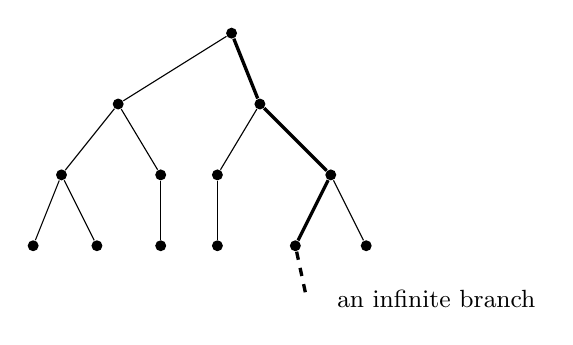
\begin{tikzpicture}[scale=0.9]
    \tikzstyle{v}=[circle, fill=black, inner sep=1.4pt]
    \node[v] (r) at (0,0) {};
    \node[v] (a) at (-1.6,-1) {};
    \node[v] (b) at (0.4,-1) {};
    \node[v] (a1) at (-2.4,-2) {};
    \node[v] (a2) at (-1.0,-2) {};
    \node[v] (b1) at (-0.2,-2) {};
    \node[v] (b2) at (1.4,-2) {};
    \node[v] (c1) at (-2.8,-3) {};
    \node[v] (c2) at (-1.9,-3) {};
    \node[v] (c3) at (-1.0,-3) {};
    \node[v] (c4) at (-0.2,-3) {};
    \node[v] (c5) at (0.9,-3) {};
    \node[v] (c6) at (1.9,-3) {};
    \draw (r) -- (a); \draw (r) -- (b);
    \draw (a) -- (a1); \draw (a) -- (a2);
    \draw (b) -- (b1); \draw (b) -- (b2);
    \draw (a1) -- (c1); \draw (a1) -- (c2);
    \draw (a2) -- (c3);
    \draw (b1) -- (c4);
    \draw (b2) -- (c5); \draw (b2) -- (c6);
    \draw[very thick] (r) -- (b) -- (b2) -- (c5);
    \draw[very thick, dashed] (c5) -- (1.05,-3.7);
    \node[right] at (1.35,-3.75) {\small an infinite branch};
  \end{tikzpicture}
\end{center}

Finally, in propositional logic we can settle the decision problem completely.

\begin{theorem}[Decidability]
  Let $S \subseteq L$ be finite and $t \in L$. Then there is an algorithm to decide, in finite time, whether $S \vdash t$.
\end{theorem}
\begin{proof}
  By completeness it is enough to decide whether $S \models t$, and only the finitely many primitives appearing in $S \cup \{t\}$ matter. So we simply draw the truth table, which has finitely many rows.
\end{proof}

Searching for a proof directly would give no such algorithm, since there are infinitely many candidate proofs; it is completeness that converts the problem into a finite one. We will see in Section~\ref{sec:predicate} that the corresponding question for predicate logic has no such easy answer, and in Section~\ref{sec:incompleteness} that some closely related questions have no algorithm at all.

\section{Well-Orderings and Ordinals}

We now jump away from logic for a while and look at some set theory. Everything in this section is really about a single idea: we want to be able to do induction and recursion along things much longer than $\N$, and the orderings that let us do that are the well-orderings.

\subsection{Well-Orderings}

\begin{definition}[Total Order]
  A \vocab{total order} (or \vocab{linear order}) is a pair $(X, <)$ where $X$ is a set and $<$ is a relation on $X$ that is
  \begin{enumerate}[label=(\roman*)]
    \item \emph{irreflexive}: for all $x \in X$, $x \not< x$;
    \item \emph{transitive}: for all $x, y, z \in X$, $x < y$ and $y < z$ implies $x < z$;
    \item \emph{trichotomous}: for all $x, y \in X$, exactly one of $x < y$, $y < x$, $x = y$ holds.
  \end{enumerate}
\end{definition}

We use the standard notation $y > x$ for $x < y$, and $x \leq y$ for `$x < y$ or $x = y$'. We could instead have defined a total order in terms of $\leq$ in the obvious way, with reflexivity, transitivity, antisymmetry and trichotomy.

\begin{example}[Total Orders]
  Each of $(\N, <)$, $(\Z, <)$, $(\Q, <)$ and $(\R, <)$ is a total order. On the other hand $(\N^+, \text{`divides'})$ is not one, as neither of $2$, $3$ divides the other, and nor is $(\mathcal{P}(S), \subseteq)$ once $|S| \geq 2$.
\end{example}

\begin{definition}[Well-Ordering]
  A total order $(X, <)$ is a \vocab{well-ordering} if every non-empty subset of $X$ has a least element.
\end{definition}

\begin{example}[Well-Orderings and Non-Examples]
  $(\N, <)$ is a well-ordering. $(\Z, <)$, $(\Q, <)$ and $(\R, <)$ are not, since $\Z$ itself, or $(0,1) \subseteq \R$, has no least element. The set $\{1/2, 2/3, 3/4, \dots\} \subseteq \R$ \emph{is} well-ordered (it has order type $\omega$, in the language below), and so is $\{1/2, 2/3, \dots\} \cup \{1\}$, where the extra point sits above everything else. But $\{\dots, -1/3, -1/2, -1\} \subseteq \R$ is not, having no least element at all.
\end{example}

\begin{center}
  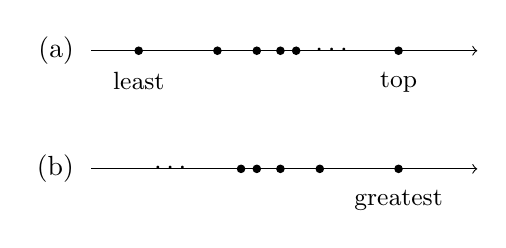
\begin{tikzpicture}[scale=1]
    \tikzstyle{v}=[circle, fill=black, inner sep=1.1pt]
    % (a) a well-ordering
    \draw[->] (-0.3,1.5) -- (4.6,1.5);
    \foreach \i in {0,...,4} {\node[v] at ({0.3 + 3.0*(1 - 1/(1+0.5*\i))},1.5) {};}
    \node at (2.75,1.5) {$\cdots$};
    \node[v] at (3.6,1.5) {};
    \node[below] at (0.3,1.35) {\small least};
    \node[below] at (3.6,1.35) {\small top};
    \node[left] at (-0.4,1.5) {(a)};
    % (b) not a well-ordering
    \draw[->] (-0.3,0) -- (4.6,0);
    \foreach \i in {0,...,4} {\node[v] at ({3.6 - 3.0*(1 - 1/(1+0.5*\i))},0) {};}
    \node at (0.7,0) {$\cdots$};
    \node[below] at (3.6,-0.15) {\small greatest};
    \node[left] at (-0.4,0) {(b)};
  \end{tikzpicture}
\end{center}

In (a) above every non-empty subset has a least element, and the order type is $\omega + 1$; in (b) the whole set has no least element, so this is not a well-ordering, even though it is a perfectly good total order. The difference is exactly that in (b) we can descend forever.

\begin{proposition}[Descending Sequence Criterion]
  A total order $(X, <)$ is a well-ordering if and only if there is no infinite strictly decreasing sequence $x_1 > x_2 > \cdots$ in $X$.
\end{proposition}
\begin{proof}
  If $x_1 > x_2 > \cdots$ is such a sequence then $\{x_1, x_2, \dots\}$ has no least element. Conversely, if $S \subseteq X$ is non-empty with no least element, pick $x_1 \in S$; as $x_1$ is not least there is $x_2 \in S$ with $x_2 < x_1$, and continuing gives an infinite decreasing sequence.
\end{proof}

The reverse direction of this used the axiom of choice, in that we chose each $x_{n+1}$ from an infinite supply of candidates. This is one of only a handful of places in this section where choice appears, and we will discuss the axiom itself properly in Section~\ref{sec:zorn}.

The point of well-orderings is that they support induction.

\begin{proposition}[Principle of Induction]\label{prop:woinduction}
  Let $X$ be a well-ordering and let $S \subseteq X$ be such that whenever $y \in S$ for all $y < x$, we have $x \in S$. Then $S = X$.

  Equivalently, if $p$ is a property such that $p(y)$ holding for all $y < x$ implies $p(x)$, then $p(x)$ holds for all $x \in X$.
\end{proposition}
\begin{proof}
  Suppose $S \neq X$. Then $X \setminus S$ is non-empty, so it has a least element $x$. Then every $y < x$ lies in $S$, so $x \in S$ by hypothesis, a contradiction.
\end{proof}

Note that there is no separate base case: the case $x = \min X$ is the case where the hypothesis `$y \in S$ for all $y < x$' is vacuous.

We will want to regard well-orderings that look the same as being the same.

\begin{definition}[Order Isomorphism]
  Two total orders $X$ and $Y$ are \vocab{order isomorphic} if there is a bijection $f: X \rightarrow Y$ with $x < y \iff f(x) < f(y)$. We call such an $f$ an \vocab{isomorphism}.
\end{definition}

For general total orders there can be many isomorphisms between two orders -- consider $\Z \to \Z$, $x \mapsto x + n$. For well-orderings this cannot happen, which is the first sign of how rigid they are.

\begin{proposition}[Uniqueness of Isomorphisms]\label{prop:uniqueiso}
  Let $X, Y$ be isomorphic well-orderings. Then there is a unique isomorphism between them.
\end{proposition}
\begin{proof}
  Let $f, g: X \rightarrow Y$ be isomorphisms. We show $f(x) = g(x)$ for all $x$ by induction on $x$, using Proposition~\ref{prop:woinduction}.

  So suppose $f(y) = g(y)$ for all $y < x$, and let $S = \{f(y) \mid y < x\}$, which by assumption equals $\{g(y) \mid y < x\}$. As $f$ is an order isomorphism, $f(x)$ is not in $S$, so $Y \setminus S$ is non-empty and has a least element $a$. Now every element of $Y$ below $f(x)$ is of the form $f(y)$ with $y < x$, so lies in $S$; hence $f(x) = a$. The identical argument gives $g(x) = a$, so $f(x) = g(x)$.
\end{proof}

\subsection{Initial Segments and Recursion}

Given an ordered set we can chop off the end and keep the beginning. What we are left with is an initial segment.

\begin{definition}[Initial Segment]
  A subset $I$ of a totally ordered set $X$ is an \vocab{initial segment} if $x \in I$ implies $y \in I$ for all $y < x$.
\end{definition}

For any $x \in X$, the set $I_x = \{y \in X \mid y < x\}$ is an initial segment. Not every initial segment is of this form in a general total order: in $\R$ the set $\{x \mid x \leq 3\}$ is an initial segment which is not any $I_x$, and in $\Q$ so is $\{x \mid x \leq 0 \text{ or } x^2 < 2\}$. In a well-ordering, however, this is the only shape available.

\begin{proposition}[Initial Segments of Well-Orderings]\label{prop:initialsegs}
  Every proper initial segment of a well-ordered set $X$ is of the form $I_x$ for some $x \in X$.
\end{proposition}
\begin{proof}
  Let $I \subsetneq X$ be an initial segment and let $x = \min(X \setminus I)$. If $y < x$ then $y \in I$ by minimality of $x$, and if $y \in I$ then $y < x$, since $y \geq x$ would put $x \in I$. So $I = I_x$.
\end{proof}

We would now like to show that every subset of a well-ordering $X$ is isomorphic to an initial segment of $X$. To construct the isomorphism we need to be able to define functions by recursion along $X$, which is the following theorem. Here $\mathcal{P}(X \times Y)$ is being used as `the set of all partial functions and more', and $G$ should be thought of as a rule telling us what to do next given everything we have done so far.

\begin{theorem}[Definition by Recursion]\label{thm:worecursion}
Let $X$ be a well-ordering, let $Y$ be a set, and let $G: \mathcal{P}(X \times Y) \rightarrow Y$ be any function. Then there is a unique function $f: X \rightarrow Y$ such that
$$f(x) = G\left(\left.f\right|_{I_x}\right) \quad \text{for all } x \in X.$$
\end{theorem}
\begin{proof}
Say that $h$ is an \emph{attempt} if $h : I \rightarrow Y$ for some initial segment $I$ of $X$, and $h(x) = G(h|_{I_x})$ for all $x \in I$.

If $h, h'$ are attempts both defined at $x$, then $h(x) = h'(x)$, by induction on $x$: if they agree below $x$ then $h|_{I_x} = h'|_{I_x}$, so $h(x) = G(h|_{I_x}) = G(h'|_{I_x}) = h'(x)$.

Next, for every $x$ there \emph{is} an attempt defined at $x$, again by induction on $x$. Indeed, suppose for each $y < x$ there is an attempt $h_y$ defined at $y$. Let $h = \bigcup_{y<x} h_y$; by the previous paragraph the $h_y$ agree wherever two of them are defined, so $h$ is a function, and it is an attempt with domain $I_x$. Then $h' = h \cup \{(x, G(h))\}$ is an attempt defined at $x$.

So we may define $f: X \to Y$ by letting $f(x)$ be the common value $h(x)$ over all attempts $h$ defined at $x$. This is well-defined by the first paragraph, and satisfies the recursion by construction.

For uniqueness, if $f, f'$ both satisfy the recursion and agree below $x$, then $f(x) = G(f|_{I_x}) = G(f'|_{I_x}) = f'(x)$, so $f = f'$ by induction.
\end{proof}

Before proving the result we were after, here is a small lemma that we will use several times.

\begin{lemma}\label{lem:orderpreservingup}
  Let $X$ be a well-ordering and $f: X \to X$ order-preserving. Then $f(x) \geq x$ for all $x \in X$.
\end{lemma}
\begin{proof}
  If not, take the least $x$ with $f(x) < x$. Applying $f$ gives $f(f(x)) < f(x)$, so $f(x)$ is a smaller counterexample, contradicting minimality.
\end{proof}

\begin{corollary}\label{cor:notpropersegment}
  A well-ordering $X$ is never isomorphic to a proper initial segment of itself.
\end{corollary}
\begin{proof}
  Suppose $f : X \to I_x$ is an isomorphism, where $I_x$ is a proper initial segment. Regarding $f$ as an order-preserving map $X \to X$, Lemma~\ref{lem:orderpreservingup} gives $f(x) \geq x$. But $f(x) \in I_x$, so $f(x) < x$, a contradiction.
\end{proof}

Now we can prove our result, by recursively sending the least unused element to the least unused element.

\begin{proposition}[Subset Collapse]\label{prop:subsetcollapse}
  Any subset $Y$ of a well-ordering $X$ is isomorphic to a unique initial segment of $X$.
\end{proposition}
\begin{proof}
  If $f: Y \to X$ is to be an order-preserving bijection onto an initial segment of $X$, then it must send each $x$ to the least element not yet used, that is,
  $$f(x) = \min\bigl(X \setminus \{f(y) \mid y \in Y, \, y < x\}\bigr).$$
  So define $f$ by this recursion; it is well-defined, since one shows by induction that $f(y) \leq y$ for all $y$, and hence $x$ itself lies in the set we are minimising over, so that set is non-empty.

  This $f$ is order-preserving: if $y < x$ then $f(y)$ is the minimum of a set containing everything $f(x)$ is minimised over, and $f(y)$ itself is excluded from the latter, so $f(y) < f(x)$. Its image is an initial segment: if $z < f(x)$ then $z$ is not in the set we minimised over to get $f(x)$, so $z = f(y)$ for some $y < x$. Finally, uniqueness of the initial segment follows from Corollary~\ref{cor:notpropersegment}: two distinct initial segments of $X$ are never isomorphic, since one is a proper initial segment of the other.
\end{proof}

\subsection{Comparing Well-Orderings}

We now know enough to compare any two well-orderings.

\begin{definition}[Comparing Well-Orderings]
  For well-orderings $X, Y$ we write $X \leq Y$ if $X$ is isomorphic to an initial segment of $Y$, and $X < Y$ if moreover $X$ is not isomorphic to $Y$ (equivalently, if $X$ is isomorphic to a \emph{proper} initial segment of $Y$).
\end{definition}

By subset collapse, $X \leq Y$ if and only if $X$ is isomorphic to \emph{some subset} of $Y$, which is often the easier condition to check.

\begin{proposition}[Trichotomy for Well-Orderings]\label{prop:wotrichotomy}
  Let $X$ and $Y$ be well-orderings. Then $X \leq Y$ or $Y \leq X$; and if both, then $X$ and $Y$ are isomorphic.
\end{proposition}
\begin{proof}
  Consider $f: X \rightarrow Y$ defined by recursion by $f(x) = \min (Y \setminus \{f(y) \mid y < x\})$. There are two cases. If $f$ is everywhere defined, then exactly as in Proposition~\ref{prop:subsetcollapse} it is an isomorphism from $X$ onto an initial segment of $Y$, so $X \leq Y$. Otherwise there is a least $x$ at which the recipe fails, meaning $\{f(y) \mid y < x\} = Y$; but then $f$ restricted to $I_x$ is an isomorphism $I_x \to Y$, so $Y \leq X$.

  Now suppose both $X \leq Y$ and $Y \leq X$, via isomorphisms $f$ onto an initial segment of $Y$ and $g$ onto an initial segment of $X$. Then $g \circ f$ is an isomorphism of $X$ onto an initial segment of $X$, which by Corollary~\ref{cor:notpropersegment} must be all of $X$. So $g \circ f$ is onto $X$, forcing $g$ to be onto $X$, and hence $g$ (and likewise $f$) is an isomorphism.
\end{proof}

\subsection{Constructing Larger Well-Orderings}

Given some well-orderings, there are two natural ways to build a longer one: add an element at the top, or stack a nested family of them.

\begin{definition}[Successor]
  Given a well-ordering $X$, choose some $x \notin X$ and well-order $X \cup \{x\}$ by setting $y < x$ for all $y \in X$. This is the \vocab{successor} of $X$, written $X^+$.
\end{definition}

Clearly $X^+$ is a well-ordering (any non-empty subset either meets $X$, and takes its least element there, or is $\{x\}$) and $X < X^+$, since $X = I_x$ inside $X^+$.

\begin{definition}[Extensions and Nested Families]
  Given well-orderings $(X, <_X)$ and $(Y, <_Y)$, we say $Y$ \vocab{extends} $X$ if $X$ is an initial segment of $Y$ and $<_X$, $<_Y$ agree where both are defined.

  A family of well-orderings $\{X_i \mid i \in I\}$ is \vocab{nested} if for all $i, j$, one of $X_i$, $X_j$ extends the other.
\end{definition}

\begin{proposition}[Unions of Nested Well-Orderings]\label{prop:nestedunion}
  Let $\{X_i \mid i \in I\}$ be a nested family of well-orderings. Then there is a well-ordering $X$ with $X_i \leq X$ for all $i$.
\end{proposition}
\begin{proof}
  Let $X = \bigcup_i X_i$ with the ordering $<_X = \bigcup_i <_i$; that is, $x < y$ in $X$ if $x, y \in X_i$ and $x <_i y$ for some $i$. Nestedness makes this a well-defined total order.

  Given non-empty $S \subseteq X$, we have $S \cap X_i \neq \emptyset$ for some $i$; let $x$ be its least element under $<_i$. Then $x$ is least in all of $S$: any $y \in S$ with $y < x$ would lie in $X_i$, since $X_i$ is an initial segment of $X$ by nestedness, and then $y \in S \cap X_i$ contradicts minimality. So $X$ is a well-ordering, and each $X_i$ is an initial segment of it.
\end{proof}

\subsection{Ordinals}

It is inconvenient to keep saying `a well-ordering, up to isomorphism'. So we give these isomorphism classes a name.

\begin{definition}[Ordinal]
  An \vocab{ordinal} is a well-ordered set, where we regard two ordinals as equal if they are isomorphic.
\end{definition}

This is a definition to be taken in a slightly informal spirit -- the isomorphism class of a well-ordering is far too big to be a set. In Section~\ref{sec:settheory} we will give a genuine definition inside $\ZF$ (an ordinal is a transitive set totally ordered by $\in$) and check it does the same job. For now, nothing we say will depend on the difference.

\begin{definition}[Order Type]
  If a well-ordering $X$ corresponds to the ordinal $\alpha$, we say $X$ has \vocab{order type} $\alpha$, and write $\otp(X) = \alpha$.
\end{definition}

The order type of the unique well-ordering on a set of $k \in \N$ points is called $k$, and the order type of $(\N, <)$ is called $\omega$.

\begin{example}[Order Types]
  In $\R$, the subset $\{-2, 3, \pi, 5\}$ has order type $4$, the subset $\{1/2, 2/3, 3/4, \dots\}$ has order type $\omega$, and $\{1/2, 2/3, \dots\} \cup \{1\}$ has order type $\omega + 1$ (a copy of $\omega$ with one extra point on top).
\end{example}

\begin{example}[Countable Ordinals Live Inside $\Q$]
  Every countable ordinal is the order type of a subset of $\Q$. Indeed, if $\alpha$ is countable then $I_\alpha$ is a countable well-ordering, and one may embed it into $\Q$ by recursion: having placed $I_\beta$ inside $\Q$, place $\beta$ above everything used so far if there is room, and otherwise squeeze it into a gap, which density allows. So the enormous ordinals of the previous list all fit inside the rationals -- what changes as we ascend is not the size of the set but the shape of the ordering.
\end{example}

For ordinals $\alpha, \beta$ we write $\alpha \leq \beta$ if $X \leq Y$ for some (equivalently, any) $X$ of order type $\alpha$ and $Y$ of order type $\beta$; this is well-defined since any two representatives are isomorphic. Proposition~\ref{prop:wotrichotomy} says that any two ordinals are comparable, and that $\alpha \leq \beta \leq \alpha$ implies $\alpha = \beta$. We also write $\alpha^+$ for the order type of $X^+$.

\begin{proposition}[$I_\alpha$ Has Order Type $\alpha$]\label{prop:Ialpha}
  For any ordinal $\alpha$, the ordinals $\beta < \alpha$ form a set $I_\alpha = \{\beta \mid \beta < \alpha\}$, well-ordered by $<$, of order type $\alpha$.
\end{proposition}
\begin{proof}
  Let $X$ be a well-ordering with $\otp(X) = \alpha$. The well-orderings which are $< X$ are precisely, up to isomorphism, the proper initial segments of $X$, which by Proposition~\ref{prop:initialsegs} are exactly the $I_x$ for $x \in X$. Distinct $x$ give non-isomorphic $I_x$ by Corollary~\ref{cor:notpropersegment}, so $x \mapsto \otp(I_x)$ is an order-preserving bijection from $X$ to $I_\alpha$.
\end{proof}

\begin{proposition}[The Ordinals are Well-Ordered]\label{prop:ordinalswo}
  Every non-empty set $S$ of ordinals has a least element.
\end{proposition}
\begin{proof}
  Choose $\alpha \in S$. If $\alpha$ is least in $S$ we are done. Otherwise $S \cap I_\alpha$ is non-empty, and $I_\alpha$ is well-ordered by Proposition~\ref{prop:Ialpha}, so it has a least element $\beta$. Any $\gamma \in S$ has $\gamma \geq \alpha > \beta$ or $\gamma \in I_\alpha$, in which case $\gamma \geq \beta$. So $\beta$ is least in $S$.
\end{proof}

So the ordinals behave in every respect like a well-ordering. They cannot literally be one, however.

\begin{theorem}[Burali-Forti Paradox]
  The ordinals do not form a set.
\end{theorem}
\begin{proof}
  Suppose $X$ were the set of all ordinals. By Proposition~\ref{prop:ordinalswo} it is well-ordered, so it has an order type, say $\alpha$. But then $X$ is isomorphic to $I_\alpha$ by Proposition~\ref{prop:Ialpha}, which is a proper initial segment of $X$ (it omits $\alpha$), contradicting Corollary~\ref{cor:notpropersegment}.
\end{proof}

This is not a paradox in the sense of an inconsistency -- it is a theorem, and a useful one. We will write $\on$ for the class of all ordinals, and treat statements about it as abbreviations, exactly as we will do for classes in general in Section~\ref{sec:settheory}.

\begin{definition}[Supremum]
  Let $S = \{\alpha_i \mid i \in I\}$ be a set of ordinals. Then $\sup S$ is the least upper bound of $S$.
\end{definition}

This exists: applying Proposition~\ref{prop:nestedunion} to the nested family $\{I_{\alpha_i}\}$ gives an upper bound $\alpha$, and then the set of upper bounds which are $\leq \alpha$ is a non-empty subset of $I_{\alpha}^+$, so has a least element by Proposition~\ref{prop:ordinalswo}. For example $\sup\{2, 4, 6, \dots\} = \omega$, and $\sup\{\alpha\} = \alpha$.

\subsection{Some Ordinals}

We know $0, 1, 2, \dots$ and $\omega$. Writing $\alpha + 1$ for $\alpha^+$, the successor and supremum operations already let us generate a great many ordinals:
$$\omega + 1, \, \omega+2, \, \dots, \, \omega + \omega = \omega \cdot 2, \, \omega\cdot 2 + 1, \, \dots, \, \omega \cdot 3, \, \dots, \, \omega \cdot \omega = \omega^2, \dots$$
where each `$\dots$' is resolved by taking a supremum, for instance $\omega \cdot 2 = \sup\{\omega, \omega + 1, \omega + 2, \dots\}$ and $\omega^2 = \sup\{\omega, \omega\cdot 2, \omega \cdot 3, \dots\}$. The notation is justified in Section~\ref{sec:ordarith}. Carrying on:

\begin{center}
  \small
  \begin{tabular}{cccccc}
    $0$ & $\omega\cdot 2 + 1$ & $\omega^2 + 1$ & $\omega^2\cdot 3$ & $\omega^{\omega + 2}$ & $\varepsilon_0 + 1$ \\
    $1$ & $\omega\cdot 2 + 2$ & $\omega^2 + 2$ & $\omega^2\cdot 4$ & $\vdots$ & $\vdots$ \\
    $2$ & $\omega\cdot 2 + 3$ & $\omega^2 + 3$ & $\omega^2\cdot 5$ & $\omega^{\omega \cdot 2}$ & $\varepsilon_0 \cdot 2$ \\
    $\vdots$ & $\vdots$ & $\vdots$ & $\vdots$ & $\vdots$ & $\vdots$ \\
    $\omega$ & $\omega\cdot 3$ & $\omega^2 + \omega$ & $\omega^3$ & $\omega^{\omega^2}$ & $\varepsilon_0^2$ \\
    $\omega + 1$ & $\omega\cdot 4$ & $\vdots$ & $\vdots$ & $\vdots$ & $\vdots$ \\
    $\omega + 2$ & $\omega\cdot 5$ & $\omega^2 + \omega \cdot 2$ & $\omega^\omega$ & $\omega^{\omega^{\omega}}$ & $\varepsilon_0^{\varepsilon_0}$ \\
    $\vdots$ & $\vdots$ & $\vdots$ & $\vdots$ & $\vdots$ & $\vdots$ \\
    $\omega + \omega$ & $\omega\cdot \omega $ & $\omega^2 \cdot 2$ & $\omega^{\omega + 1}$ & $\omega^{\omega^{.^{.^.}}}$ & $\varepsilon_0^{\varepsilon_0^{.^{.^.}}}$ \\
    $=\omega\cdot 2$ & $=\omega^2$ & &  & $= \varepsilon_0$ & $= \varepsilon_1$ \\
  \end{tabular}
\end{center}

It helps to have a picture. Drawing each ordinal as a point on a line, with the tick marks bunching up as we approach a limit, the beginning of the list looks like this.

\begin{center}
  \begin{tikzpicture}[scale=1]
    \draw (-0.2,0) -- (12.2,0);
    \foreach \b in {0.4, 3.2, 6.0, 8.8} {
      \foreach \i in {0,...,4} {
        \draw ({\b + 2.4*(1 - 1/(1+0.6*\i))},-0.11) -- ({\b + 2.4*(1 - 1/(1+0.6*\i))},0.11);
      }
    }
    \node at (11.35,0) {$\cdots$};
    \foreach \b/\l in {0.4/{$0$}, 3.2/{$\omega$}, 6.0/{$\omega\cdot 2$}, 8.8/{$\omega\cdot 3$}} {
      \draw[dashed] (\b,-0.2) -- (\b,0.55);
      \node[above] at (\b,0.5) {\small \l};
    }
    \draw[dashed] (12.0,-0.2) -- (12.0,0.55);
    \draw (12.0,-0.11) -- (12.0,0.11);
    \node[above] at (12.0,0.5) {\small $\omega^2$};
  \end{tikzpicture}
\end{center}

Every ordinal in the table above is \emph{countable}: at each step we either add one element or take a countable supremum of countable ordinals, and a countable union of countable sets is countable. It is natural to ask whether we ever escape. Since a well-ordering of a set $X$ of order type $\alpha$ is the same thing as an injection of $X$ into $I_\alpha$ hitting an initial segment, this is essentially the question of whether we can well-order $\R$. The answer is yes, and remarkably we can prove it without ever writing such an ordering down.

\subsection{Uncountable Ordinals and Hartogs' Lemma}

\begin{theorem}[Existence of an Uncountable Ordinal]\label{thm:omega1}
  There is an uncountable ordinal.
\end{theorem}
\begin{proof}
  Let
  $$A = \{R \in \mathcal{P}(\omega \times \omega) \mid R \text{ is a well-ordering of a subset of } \omega\},$$
  which is a set by separation from $\mathcal{P}(\omega\times\omega)$. Then $B = \{\otp(R) \mid R \in A\}$ is a set (it is the image of $A$ under a function-class, using replacement, which we discuss in Section~\ref{sec:settheory}), and $B$ is precisely the set of all countable ordinals -- every countable ordinal is the order type of a well-ordering of a subset of $\omega$, and conversely.

  Let $\omega_1 = \sup B$. If $\omega_1$ were countable then $\omega_1 \in B$, and so $\omega_1^+ \in B$ as well (a successor of a countable ordinal is countable), giving $\omega_1^+ \leq \sup B = \omega_1$, which is absurd. So $\omega_1$ is uncountable.
\end{proof}

Alternatively, and more slickly: $B$ cannot be all of the ordinals, since the ordinals do not form a set, so some ordinal is uncountable.

By construction $\omega_1$ is the \emph{least} uncountable ordinal, and it has some remarkable properties. Every proper initial segment $I_\alpha$ of $\omega_1$ is countable, while $\omega_1$ itself is not; so $\omega_1$ is uncountable but is `built out of' countable pieces. Also, every sequence $\alpha_1, \alpha_2, \dots$ of ordinals below $\omega_1$ is bounded below $\omega_1$, namely by $\sup\{\alpha_1, \alpha_2, \dots\}$, which is countable as a countable union of countable sets. So $\omega_1$ cannot be reached from below by any sequence -- it is very far from being $\omega$.

The same argument, run with an arbitrary set in place of $\omega$, gives the following, which is the workhorse of the next section.

\begin{theorem}[Hartogs' Lemma]\label{thm:hartogs}
  For every set $X$ there is an ordinal $\alpha$ that does not inject into $X$. The least such ordinal is written $\gamma(X)$, read `\vocab{Hartogs' ordinal} of $X$'.
\end{theorem}
\begin{proof}
  Let $A$ be the set of pairs $(Y, R)$ with $Y \subseteq X$ and $R$ a well-ordering of $Y$; this is a set, being a subset of $\mathcal{P}(X) \times \mathcal{P}(X \times X)$. Let $B = \{\otp(R) \mid (Y, R) \in A\}$, a set by replacement, and let $\gamma = \sup\{\beta^+ \mid \beta \in B\}$.

  If $\gamma$ injected into $X$, say with image $Y$, then transporting the ordering of $I_\gamma$ across gives a well-ordering of $Y \subseteq X$ of order type $\gamma$, so $\gamma \in B$ and hence $\gamma^+ \leq \gamma$, a contradiction. So $\gamma$ does not inject into $X$, and by Proposition~\ref{prop:ordinalswo} there is a least such ordinal.
\end{proof}

So $\gamma(\omega) = \omega_1$. Note that $\gamma(X)$ is a genuine `size barrier' for $X$: no ordinal $\geq \gamma(X)$ injects into $X$ either, since it has $\gamma(X)$ as an initial segment.

\subsection{Successors and Limits}

Ordinals come in two flavours.

\begin{definition}[Limits and Successors]
  An ordinal $\alpha$ is a \vocab{successor} if $\alpha = \beta^+$ for some ordinal $\beta$. Otherwise $\alpha$ is a \vocab{limit}.
\end{definition}

An ordinal (viewed as a well-ordered set $I_\alpha$) has a greatest element if and only if it is a successor. So $\alpha$ is a limit precisely when it has no greatest element, and then $\alpha = \sup I_\alpha$. We typically write $\lambda$ for a limit ordinal.

\begin{example}
  $5 = 4^+$ is a successor, and $\omega + 2 = (\omega^+)^+$ is a successor. Both $\omega$ and $\omega \cdot 2$ are limits, as is $0$ (vacuously -- it is not a successor of anything). This is why the clause for limits in the recursive definitions below always says `non-zero limit'.
\end{example}

Consequently, when defining something by recursion on the ordinals we give three clauses: the value at $0$, the value at $\alpha^+$ in terms of the value at $\alpha$, and the value at a non-zero limit $\lambda$ in terms of the values below $\lambda$. This is \vocab{transfinite recursion}, and it is justified by Theorem~\ref{thm:worecursion} applied to $I_\beta$ for each $\beta$ (we cannot recurse on `all the ordinals' at once, since they do not form a set, so officially we define the function on $I_\beta$ for each $\beta$ and use uniqueness to glue).

\subsection{Ordinal Arithmetic}\label{sec:ordarith}

We now make formal sense of the notation $\omega + \omega$, $\omega \cdot 2$ and so on used above.

\begin{definition}[Ordinal Addition, Inductive]
We define $\alpha + \beta$ by recursion on $\beta$, keeping $\alpha$ fixed:
\begin{align*}
  \alpha + 0 &= \alpha,\\
  \alpha + \beta^+ &= (\alpha + \beta)^+,\\
  \alpha + \lambda &= \sup\{\alpha + \gamma \mid \gamma < \lambda\} \quad \text{for } \lambda \text{ a non-zero limit.}
\end{align*}
\end{definition}

\begin{proposition}[Addition is Not Commutative]
  We have $1 + \omega \neq \omega + 1$.
\end{proposition}
\begin{proof}
  On one hand $\omega + 1 = \omega + 0^+ = (\omega + 0)^+ = \omega^+$. On the other hand, $\omega$ is a non-zero limit, so $1 + \omega = \sup\{1 + n \mid n < \omega\} = \sup\{1, 2, 3, \dots\} = \omega$. And $\omega < \omega^+$.
\end{proof}

The asymmetry comes from our decision to recurse on the right-hand argument. Addition is, however, associative.

\begin{proposition}[Addition is Associative]
  For all ordinals $\alpha, \beta, \gamma$ we have $\alpha + (\beta + \gamma) = (\alpha + \beta) + \gamma$.
\end{proposition}
\begin{proof}
We induct on $\gamma$, keeping $\alpha, \beta$ fixed. If $\gamma = 0$ then $\alpha+(\beta+0) = \alpha+\beta = (\alpha+\beta)+0$.

If $\gamma = \delta^+$ is a successor, then
\begin{align*}
  \alpha + (\beta + \delta^+) = \alpha + (\beta + \delta)^+
  = [\alpha + (\beta + \delta)]^+ = [(\alpha + \beta) + \delta]^+
  = (\alpha + \beta) + \delta^+,
\end{align*}
using the induction hypothesis in the third equality.

If $\gamma = \lambda$ is a non-zero limit, then
\begin{align*}
(\alpha+\beta)+\lambda & =\sup \{(\alpha+\beta)+\gamma \mid \gamma<\lambda\} =\sup \{\alpha+(\beta+\gamma) \mid \gamma<\lambda\}.
\end{align*}
We claim that $\beta+\lambda$ is a limit. Indeed $\beta+\lambda=\sup \{\beta+\gamma \mid \gamma<\lambda\}$, and since $\lambda$ is a limit, for every $\gamma < \lambda$ there is $\gamma'$ with $\gamma < \gamma' < \lambda$, whence $\beta + \gamma < \beta + \gamma'$. So this set has no greatest element.

Hence $\alpha + (\beta + \lambda) = \sup\{\alpha + \delta \mid \delta < \beta + \lambda\}$, and we must show
$$\sup\{\alpha + \delta \mid \delta < \beta +\lambda\} = \sup \{\alpha + (\beta + \gamma) \mid \gamma < \lambda\}.$$
Each element of the right-hand set is an element of the left-hand set (as $\beta + \gamma < \beta + \lambda$), so the left supremum is $\geq$ the right. Conversely, given $\delta < \beta + \lambda = \sup\{\beta + \gamma \mid \gamma < \lambda\}$ we have $\delta < \beta + \gamma$ for some $\gamma < \lambda$, so $\alpha + \delta \leq \alpha + (\beta+\gamma)$. So the left supremum is $\leq$ the right, and they are equal.
\end{proof}

There is an alternative definition of addition in terms of actual well-orderings, obtained by writing out all the elements of $\alpha$ and then all the elements of $\beta$ after them:
\[
  \alpha + \beta = \underbrace{\quad\quad\vphantom{\beta}\alpha\vphantom{\beta}\quad\quad}\underbrace{\quad\;\beta\;\quad}
\]

\begin{definition}[Ordinal Addition, Synthetic]
  $\alpha + \beta$ is the order type of $\alpha \sqcup \beta$ (say $\alpha \times \{0\} \cup \beta \times \{1\}$) with all of $\alpha$ before all of $\beta$.
\end{definition}

From this picture, associativity is immediate, and it is obvious why $1 + \omega = \omega$ (a dot followed by $\omega$ dots is just $\omega$ dots) while $\omega + 1 \neq \omega$ ($\omega$ dots followed by a dot has a greatest element). Reassuringly, the two definitions agree.

\begin{proposition}[The Two Definitions of Addition Agree]
  The inductive and synthetic definitions of addition coincide.
\end{proposition}
\begin{proof}
We write $+$ for the inductive definition and $+'$ for the synthetic one, and induct on $\beta$ with $\alpha$ fixed.
\begin{enumerate}[label=(\roman*)]
  \item \emph{Zero}: $\alpha + 0 = \alpha = \alpha +' 0$.
  \item \emph{Successor}: $\alpha + \beta^+ = (\alpha + \beta)^+ = (\alpha +' \beta)^+$, which is the order type of
  $$
  \underbrace{\quad\quad\vphantom{\beta}\alpha\vphantom{\beta}\quad\quad}\underbrace{\quad\;\beta\;\quad}
  \underbrace{\vphantom{\beta}\bullet\vphantom{\beta}}
  $$
  and that is precisely $\alpha +' \beta^+$.
  \item \emph{Non-zero limit}: $\alpha + \lambda = \sup\{\alpha + \gamma \mid \gamma < \lambda\} = \sup\{\alpha +' \gamma \mid \gamma < \lambda\} = \alpha +' \lambda$, where the last step is because the well-orderings $\alpha \sqcup \gamma$ for $\gamma < \lambda$ are nested, so their supremum is their union, which is $\alpha \sqcup \lambda$. \qedhere
\end{enumerate}
\end{proof}

Multiplication works in exactly the same way.

\begin{definition}[Ordinal Multiplication, Inductive]
  We define $\alpha \cdot \beta$ by recursion on $\beta$, keeping $\alpha$ fixed:
  \begin{align*}
    \alpha \cdot 0 &= 0, \\
    \alpha \cdot \beta^+ &= \alpha \cdot \beta + \alpha, \\
    \alpha \cdot \lambda &= \sup \{\alpha \cdot \gamma \mid \gamma < \lambda\} \quad \text{for } \lambda \text{ a non-zero limit.}
  \end{align*}
\end{definition}

\begin{definition}[Ordinal Multiplication, Synthetic]
  $\alpha \cdot \beta$ is the order type of $\alpha \times \beta$, ordered by $(x, y) < (x', y')$ if $y < y'$, or if $y = y'$ and $x < x'$.
\end{definition}

That is, $\beta$ copies of $\alpha$ laid end to end:
$$
\alpha \cdot \beta = \underbrace{
  \underbrace{\quad\alpha\quad}
  \underbrace{\quad\alpha\quad}
  \cdots
  \underbrace{\quad\alpha\quad}
}_{\beta\text{ copies}}.
$$
As with addition, the two definitions agree, by an induction identical in shape to the one above. Multiplication is associative and again not commutative, and the synthetic picture shows why very clearly.

\begin{center}
  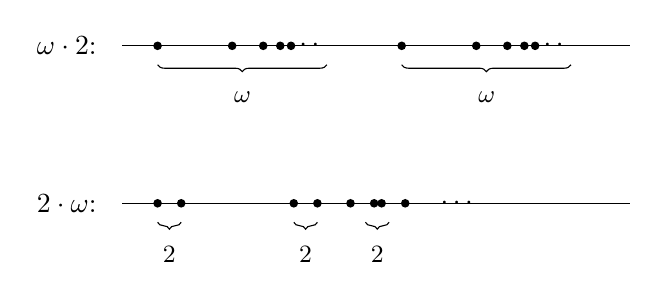
\begin{tikzpicture}[scale=1]
    \tikzstyle{v}=[circle, fill=black, inner sep=1.1pt]
    % omega . 2
    \node[left] at (-0.35, 0.9) {$\omega \cdot 2$:};
    \draw (-0.15,0.9) -- (6.3,0.9);
    \foreach \i in {0,...,4} {\node[v] at ({0.3 + 2.3*(1 - 1/(1+0.7*\i))},0.9) {};}
    \node at (2.15,0.9) {$\cdots$};
    \foreach \i in {0,...,4} {\node[v] at ({3.4 + 2.3*(1 - 1/(1+0.7*\i))},0.9) {};}
    \node at (5.25,0.9) {$\cdots$};
    \draw[decorate, decoration={brace, mirror, raise=4pt}] (0.3,0.8) -- (2.45,0.8);
    \draw[decorate, decoration={brace, mirror, raise=4pt}] (3.4,0.8) -- (5.55,0.8);
    \node at (1.38,0.25) {\small $\omega$};
    \node at (4.48,0.25) {\small $\omega$};
    % 2 . omega
    \node[left] at (-0.35, -1.1) {$2 \cdot \omega$:};
    \draw (-0.15,-1.1) -- (6.3,-1.1);
    \foreach \i in {0,...,3} {
      \node[v] at ({0.3 + 4.2*(1 - 1/(1+0.7*\i))},-1.1) {};
      \node[v] at ({0.6 + 4.2*(1 - 1/(1+0.7*\i))},-1.1) {};
    }
    \node at (4.1,-1.1) {$\cdots$};
    \foreach \x in {0.3, 2.03, 2.94} {
      \draw[decorate, decoration={brace, mirror, raise=4pt}] (\x,-1.2) -- ({\x+0.3},-1.2);
      \node at ({\x+0.15},-1.75) {\small $2$};
    }
  \end{tikzpicture}
\end{center}

Reading the top line, $\omega \cdot 2 = \omega + \omega$ is genuinely longer than $\omega$; reading the bottom line, $2 \cdot \omega$ is $\omega$ copies of a two-element set, which is just $\omega$. So $2 \cdot \omega = \omega \neq \omega \cdot 2$.

\begin{definition}[Ordinal Exponentiation]
  We define $\alpha^\beta$ by recursion on $\beta$:
  \begin{align*}
    \alpha^0 &= 1, \\
    \alpha^{\beta^+} &= \alpha^\beta \cdot \alpha, \\
    \alpha^\lambda &= \sup \{\alpha^\gamma \mid \gamma < \lambda\} \quad \text{for } \lambda \text{ a non-zero limit.}
  \end{align*}
\end{definition}

\begin{example}
  $\omega^1 = \omega^0 \cdot \omega = \omega$ and $\omega^2 = \omega \cdot \omega$, as the notation in our table suggested. But $2^\omega = \sup\{2^n \mid n < \omega\} = \sup\{1, 2, 4, 8, \dots\} = \omega$, which is countable. So ordinal exponentiation is emphatically \emph{not} cardinal exponentiation -- we will meet the latter in Section~\ref{sec:cardinals}, where $2^{\aleph_0}$ is uncountable.
\end{example}

\subsection{Normal Functions and \texorpdfstring{$\varepsilon$}{epsilon}-Numbers}

The definitions above all have the same shape: increasing, and continuous at limits. This is worth isolating.

\begin{definition}[Normal Function]
  A function $f: \on \to \on$ is \vocab{normal} if $f(\alpha) < f(\alpha^+)$ for every $\alpha$, and $f(\lambda) = \sup\{f(\gamma) \mid \gamma < \lambda\}$ for every non-zero limit $\lambda$.
\end{definition}

For example $\alpha \mapsto \beta + \alpha$ is normal for any $\beta$, and $\alpha \mapsto \beta^\alpha$ is normal for any $\beta > 1$; both are immediate from the recursive definitions.

\begin{lemma}\label{lem:normalinc}
  A normal function $f$ is strictly increasing, and satisfies $f(\alpha) \geq \alpha$ for all $\alpha$.
\end{lemma}
\begin{proof}
  For the first part, fix $\alpha$ and induct on $\beta > \alpha$. If $\beta = \alpha^+$ this is the definition. If $\beta = \gamma^+$ with $\gamma > \alpha$ then $f(\alpha) < f(\gamma) < f(\gamma^+)$ by induction. If $\beta$ is a limit then $f(\beta) = \sup\{f(\gamma) \mid \gamma < \beta\} \geq f(\alpha^+) > f(\alpha)$, as $\alpha^+ < \beta$.

  For the second, induct on $\alpha$. It is clear for $0$. For successors, $f(\alpha^+) > f(\alpha) \geq \alpha$ gives $f(\alpha^+) \geq \alpha^+$. For a non-zero limit $\lambda$, $f(\lambda) = \sup\{f(\gamma) \mid \gamma < \lambda\} \geq \sup\{\gamma \mid \gamma < \lambda\} = \lambda$.
\end{proof}

\begin{lemma}[Fixed Point Lemma]\label{lem:fixedpoint}
  Let $f$ be a normal function. Then for every ordinal $\alpha$ there is $\beta \geq \alpha$ with $f(\beta) = \beta$.
\end{lemma}
\begin{proof}
  Let $\beta = \sup\{\alpha, f(\alpha), f(f(\alpha)), \dots\}$. If the sequence is eventually constant we have found a fixed point. Otherwise the sequence is strictly increasing, so $\beta$ is a limit and
  $$f(\beta) = \sup\{f(\gamma) \mid \gamma < \beta\} = \sup\{f(\alpha), f(f(\alpha)), \dots\} = \beta,$$
  using Lemma~\ref{lem:normalinc} for the middle equality. In either case $\beta \geq \alpha$.
\end{proof}

\begin{lemma}[Division for Normal Functions]\label{lem:normaldivision}
  Let $f$ be a normal function and $\alpha$ an ordinal with $f(0) \leq \alpha$. Then there is a greatest $\gamma$ with $f(\gamma) \leq \alpha$.
\end{lemma}
\begin{proof}
  Let $\gamma = \sup\{\beta \mid f(\beta) \leq \alpha\}$, which is a supremum of a set of ordinals since all such $\beta$ satisfy $\beta \leq f(\beta) \leq \alpha$ by Lemma~\ref{lem:normalinc}. If the set has a greatest element we are done. Otherwise $\gamma$ is a limit and $f(\gamma) = \sup\{f(\beta) \mid \beta < \gamma\} \leq \alpha$, so $\gamma$ itself is the greatest such ordinal.
\end{proof}

Applying this to the normal function $\alpha \mapsto \omega^\alpha$ gives the \vocab{$\varepsilon$-numbers}: the ordinals $\varepsilon$ with $\omega^\varepsilon = \varepsilon$. The least of them is
$$\varepsilon_0 = \sup\{\omega, \omega^\omega, \omega^{\omega^\omega}, \dots\},$$
which is where the fifth column of our table was heading. There is nothing special about $\varepsilon_0$ -- since the supremum of a set of fixed points is again a fixed point, the fixed points themselves are enumerated by a normal function $\alpha \mapsto \varepsilon_\alpha$, which then has its own fixed points, and so on. All of these ordinals are still countable, and so are dwarfed by $\omega_1$.

\subsection{Further Ordinal Arithmetic}

We record a few more facts about ordinal arithmetic, all proved by inductions of the kind we have already seen, and finish with a normal form for ordinals.

\begin{proposition}[Strict Monotonicity on the Right]\label{prop:ordmono}
  Let $\alpha, \beta, \gamma$ be ordinals with $\beta < \gamma$. Then $\alpha + \beta < \alpha + \gamma$. Consequently $\alpha + \beta = \alpha + \gamma$ implies $\beta = \gamma$.
\end{proposition}
\begin{proof}
  We induct on $\gamma > \beta$. If $\gamma = \delta^+$ then $\beta \leq \delta$, so $\alpha + \beta \leq \alpha + \delta < (\alpha+\delta)^+ = \alpha + \gamma$, using the induction hypothesis if $\beta < \delta$. If $\gamma$ is a limit then $\beta^+ < \gamma$, so $\alpha + \beta < \alpha + \beta^+ \leq \sup\{\alpha + \delta \mid \delta < \gamma\} = \alpha + \gamma$.

  The cancellation statement follows since $\beta \neq \gamma$ would give $\alpha + \beta \neq \alpha + \gamma$ by trichotomy.
\end{proof}

Monotonicity on the \emph{left} is false: $1 < 2$, but $1 + \omega = 2 + \omega = \omega$. So we may cancel on the left but not on the right.

\begin{proposition}[Ordinal Subtraction]
  Let $\alpha \leq \beta$. Then there is a unique ordinal $\gamma$ with $\alpha + \gamma = \beta$.
\end{proposition}
\begin{proof}
  Take a well-ordering $Y$ of order type $\beta$. Since $\alpha \leq \beta$, there is an initial segment $I$ of $Y$ of order type $\alpha$, and we let $\gamma = \otp(Y \setminus I)$. By the synthetic definition of addition, $\alpha + \gamma = \otp(Y) = \beta$. Uniqueness is Proposition~\ref{prop:ordmono}.
\end{proof}

\begin{proposition}[Distributivity]
  For all ordinals, $\alpha \cdot (\beta + \gamma) = \alpha\cdot\beta + \alpha\cdot\gamma$.
\end{proposition}
\begin{proof}
  Use the synthetic definitions: $\alpha\cdot(\beta+\gamma)$ is $\beta + \gamma$ copies of $\alpha$ laid end to end, which is $\beta$ copies followed by $\gamma$ copies.
\end{proof}

Distributivity on the other side fails, and the smallest counterexample is a good test of the definitions: $(1 + 1)\cdot \omega = 2 \cdot \omega = \omega$, whereas $1 \cdot \omega + 1 \cdot \omega = \omega + \omega = \omega \cdot 2$.

\begin{proposition}[Division Algorithm]\label{prop:orddivision}
  Let $\alpha$ be an ordinal and $\beta > 0$. Then there are unique ordinals $\gamma$ and $\delta$ with
  $$\alpha = \beta \cdot \gamma + \delta, \qquad \delta < \beta.$$
\end{proposition}
\begin{proof}
  The map $\gamma \mapsto \beta\cdot\gamma$ is normal, so by Lemma~\ref{lem:normaldivision} there is a greatest $\gamma$ with $\beta\cdot\gamma \leq \alpha$. By subtraction there is a unique $\delta$ with $\beta\cdot\gamma + \delta = \alpha$, and $\delta < \beta$, since $\delta \geq \beta$ would give $\beta\cdot\gamma^+ = \beta\cdot\gamma + \beta \leq \alpha$, contradicting maximality of $\gamma$. Uniqueness follows from that of $\gamma$ together with Proposition~\ref{prop:ordmono}.
\end{proof}

Applying this repeatedly with $\beta$ a power of $\omega$ gives a normal form, exactly analogous to writing a natural number in base $10$.

\begin{theorem}[Cantor Normal Form]
  Every ordinal $\alpha > 0$ can be written uniquely as
  $$\alpha = \omega^{\beta_1}\cdot n_1 + \omega^{\beta_2}\cdot n_2 + \cdots + \omega^{\beta_k}\cdot n_k$$
  with $k \geq 1$, ordinals $\beta_1 > \beta_2 > \cdots > \beta_k$ and positive integers $n_1, \dots, n_k$.
\end{theorem}
\begin{proof}[Proof sketch]
  Since $\alpha \mapsto \omega^\alpha$ is normal, Lemma~\ref{lem:normaldivision} gives a greatest $\beta_1$ with $\omega^{\beta_1} \leq \alpha$. Dividing by $\omega^{\beta_1}$ using Proposition~\ref{prop:orddivision} gives $\alpha = \omega^{\beta_1}\cdot \gamma + \delta$ with $\delta < \omega^{\beta_1}$, and maximality of $\beta_1$ forces $\gamma$ to be a positive integer $n_1$. Now $\delta < \alpha$, so we may repeat; the process terminates because the ordinals $\delta$ produced are strictly decreasing, and there is no infinite strictly decreasing sequence of ordinals. Uniqueness follows by induction, using the fact that $\omega^{\beta}\cdot n < \omega^{\beta'}$ whenever $\beta < \beta'$ and $n < \omega$.
\end{proof}

\begin{example}[Arithmetic in Normal Form]
  Let us compute $(\omega^2 + \omega\cdot 3) + (\omega \cdot 2 + 5)$. Addition is associative, and $\omega\cdot 3 + \omega\cdot 2 = \omega\cdot 5$ by distributivity, so this is $\omega^2 + \omega\cdot 5 + 5$. On the other hand $(\omega + 1) \cdot \omega = \sup\{(\omega+1)\cdot n \mid n < \omega\} = \sup\{\omega, \omega\cdot 2 + 1, \omega \cdot 3 + 2, \dots\} = \omega^2$, so the $1$ is entirely swallowed. In general, when adding ordinals in normal form, every term of the left-hand ordinal of degree less than the leading degree of the right-hand one simply disappears.
\end{example}

\begin{example}
  $\omega^2 \cdot 3 + \omega \cdot 5 + 7$ is in Cantor normal form. On the other hand $\varepsilon_0$ is not expressible in this way in terms of \emph{smaller} ordinals: its normal form is $\omega^{\varepsilon_0}$, which is the statement that $\varepsilon_0$ is a fixed point of $\alpha \mapsto \omega^\alpha$. So the $\varepsilon$-numbers are precisely the ordinals which the normal form fails to simplify.
\end{example}

\section{Posets and Zorn's Lemma}\label{sec:zorn}

Well-orderings are very rigid objects. In this section we look at the opposite extreme -- orderings where elements are allowed to be incomparable -- and arrive at Zorn's lemma, which is the form in which the axiom of choice is used in practice throughout mathematics.

\subsection{Partial Orders and Hasse Diagrams}

\begin{definition}[Poset]
  A \vocab{partially ordered set}, or \vocab{poset}, is a pair $(X, \leq)$ where $X$ is a set and $\leq$ is a relation on $X$ that is reflexive, transitive and antisymmetric (if $x \leq y$ and $y \leq x$ then $x = y$). We write $x < y$ if $x \leq y$ and $x \neq y$; in terms of $<$, a poset is exactly an irreflexive transitive relation.
\end{definition}

\begin{example}[Posets]~
  \begin{enumerate}[label=(\roman*)]
    \item Any total order, for instance $(\R, \leq)$ or any well-ordering.
    \item $(\N^+, \text{`divides'})$, in which $2$ and $3$ are incomparable.
    \item For any set $S$, the power set $\mathcal{P}(S)$ ordered by $A \leq B$ if $A \subseteq B$.
    \item Any subset $X \subseteq \mathcal{P}(S)$ with the same ordering. Most of our applications will be of this form: $X$ will be the set of subsets of $S$ with some property, ordered by inclusion.
    \item The five-element poset with $a \leq b \leq c$ and $a \leq d \leq e$ and nothing else (beyond what transitivity and reflexivity force). So $a \leq c$, but $b$ and $d$ are incomparable.
  \end{enumerate}
\end{example}

Small posets are best understood by drawing them.

\begin{definition}[Hasse Diagram]
  A \vocab{Hasse diagram} of a poset $X$ consists of a drawing of the points of $X$ in the plane, with an upward line from $x$ to $y$ whenever $y$ \vocab{covers} $x$, meaning $y > x$ and there is no $z$ with $y > z > x$.
\end{definition}

Here are the poset (v) above on the left, and two more on the right.

\begin{center}
  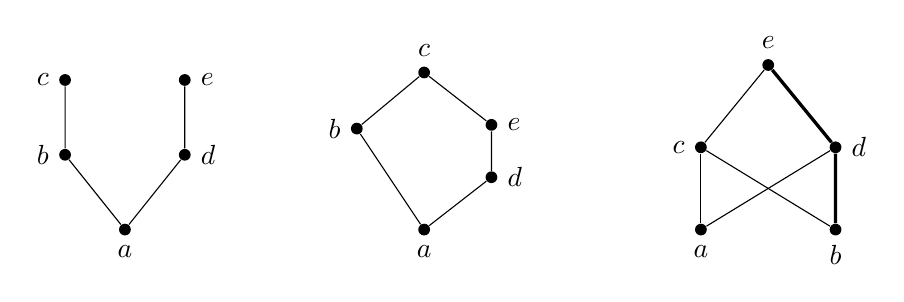
\begin{tikzpicture}[scale=0.95]
    \tikzstyle{v}=[circle, fill=black, inner sep=1.5pt]
    % poset (v)
    \node[v, label=below:{$a$}] (a) at (0,0) {};
    \node[v, label=left:{$b$}] (b) at (-0.8,1) {};
    \node[v, label=left:{$c$}] (c) at (-0.8,2) {};
    \node[v, label=right:{$d$}] (d) at (0.8,1) {};
    \node[v, label=right:{$e$}] (e) at (0.8,2) {};
    \draw (a)--(b)--(c); \draw (a)--(d)--(e);
    % second
    \begin{scope}[xshift=4cm]
      \node[v, label=below:{$a$}] (a2) at (0,0) {};
      \node[v, label=left:{$b$}] (b2) at (-0.9,1.35) {};
      \node[v, label=right:{$d$}] (d2) at (0.9,0.7) {};
      \node[v, label=right:{$e$}] (e2) at (0.9,1.4) {};
      \node[v, label=above:{$c$}] (c2) at (0,2.1) {};
      \draw (a2)--(b2)--(c2); \draw (a2)--(d2)--(e2)--(c2);
    \end{scope}
    % third, with chain highlighted
    \begin{scope}[xshift=8.6cm]
      \node[v, label=below:{$a$}] (a3) at (-0.9,0) {};
      \node[v, label=below:{$b$}] (b3) at (0.9,0) {};
      \node[v, label=left:{$c$}] (c3) at (-0.9,1.1) {};
      \node[v, label=right:{$d$}] (d3) at (0.9,1.1) {};
      \node[v, label=above:{$e$}] (e3) at (0,2.2) {};
      \draw (a3)--(c3); \draw (a3)--(d3); \draw (b3)--(c3); \draw (b3)--(d3);
      \draw (c3)--(e3); \draw (d3)--(e3);
      \draw[very thick] (b3)--(d3)--(e3);
    \end{scope}
  \end{tikzpicture}
\end{center}

The middle diagram is a warning: there is no notion of `height' or `rank' in a poset, since $b$ is covered by $c$ directly while $d$, $e$ take two steps to get from $a$ to $c$. In the right-hand diagram the thickened path $b < d < e$ is a chain, in the following sense.

\begin{definition}[Chain and Antichain]
  A subset $S$ of a poset $X$ is a \vocab{chain} if any two of its elements are comparable, that is, if $S$ is totally ordered by $\leq$. It is an \vocab{antichain} if no two distinct members of $S$ are comparable.
\end{definition}

\begin{example}
  In a total order, every subset is a chain and every antichain has at most one element. In $(\N^+, \text{`divides'})$ the set $\{1, 2, 4, 8, \dots\}$ is a chain and the set of primes is an antichain. In $\mathcal{P}(\N)$, the sets $A_x = \{q \in \Q \mid q < x\}$ for $x \in \R$ form a chain of size $2^{\aleph_0}$.
\end{example}

\begin{definition}[Upper Bound and Supremum]
  For $S \subseteq X$, an element $x \in X$ is an \vocab{upper bound} for $S$ if $y \leq x$ for all $y \in S$. It is a \vocab{least upper bound} or \vocab{supremum} for $S$ if in addition $x \leq y$ for every upper bound $y$ of $S$, and we then write $x = \sup S$.
\end{definition}

Suprema are unique when they exist, by antisymmetry.

\begin{definition}[Complete Poset]
  A poset $X$ is \vocab{complete} if every subset $S \subseteq X$ has a supremum.
\end{definition}

In a complete poset there is automatically a greatest element $\sup X$ and a least element $\sup \emptyset$ (every element is vacuously an upper bound for $\emptyset$). The example to keep in mind is $\mathcal{P}(S)$, where $\sup$ is union. Note that $(\R, \leq)$ is \emph{not} complete in this sense -- unbounded sets have no supremum -- but $[0,1]$ is.

\begin{definition}[Order-Preserving Map]
  For a poset $X$, a function $f: X \rightarrow X$ is \vocab{order-preserving} if $x \leq y$ implies $f(x) \leq f(y)$.
\end{definition}

\begin{theorem}[Knaster--Tarski Fixed Point Theorem]\label{thm:knastertarski}
  Let $X$ be a complete poset and $f: X \rightarrow X$ order-preserving. Then $f$ has a fixed point.
\end{theorem}
\begin{proof}
  Let $E = \{x \in X \mid x \leq f(x)\}$ and $s = \sup E$. We claim $f(s) = s$.

  To show $s \leq f(s)$, it is enough to show that $f(s)$ is an upper bound for $E$, since $s$ is the \emph{least} upper bound. And indeed if $x \in E$ then $x \leq s$, so $f(x) \leq f(s)$, so $x \leq f(x) \leq f(s)$.

  To show $f(s) \leq s$, it is enough to show $f(s) \in E$, since $s$ is an upper bound for $E$. But we have just shown $s \leq f(s)$, so $f(s) \leq f(f(s))$ as $f$ is order-preserving, which says exactly that $f(s) \in E$.
\end{proof}

Note that no choice, and no ordinals, were used here. As an application we get a proof of the Schr\"oder--Bernstein theorem, which we will want in Section~\ref{sec:cardinals}.

\begin{corollary}[Schr\"oder--Bernstein Theorem]\label{cor:csb}
  Let $A, B$ be sets and let $f: A \rightarrow B$ and $g: B \rightarrow A$ be injections. Then there is a bijection from $A$ to $B$.
\end{corollary}
\begin{proof}
  We aim to partition $A$ into $P$ and $Q$, and $B$ into $R$ and $S$, in such a way that $f(P) = R$ and $g(S) = Q$. Given such a partition we may define a bijection $h : A \to B$ by taking $h = f$ on $P$ and $h = g^{-1}$ on $Q$.
  \begin{center}
    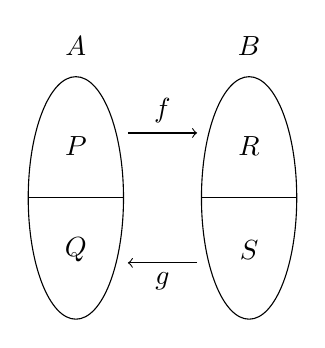
\begin{tikzpicture}[scale=1.1]
      \draw (-1, 0) ellipse (0.55 and 1.4);
      \draw (-1.55, 0) -- (-0.45, 0);
      \node at (-1, -0.6) {$Q$};
      \node at (-1, 0.6) {$P$};
      \node at (-1, 1.75) {$A$};
      \draw (1, 0) ellipse (0.55 and 1.4);
      \draw (0.45, 0) -- (1.55, 0);
      \node at (1, -0.6) {$S$};
      \node at (1, 0.6) {$R$};
      \node at (1, 1.75) {$B$};
      \draw [->] (-0.4, 0.75) -- (0.4, 0.75) node [pos = 0.5, above] {$f$};
      \draw [->] (0.4, -0.75) -- (-0.4, -0.75) node [pos = 0.5, below] {$g$};
    \end{tikzpicture}
  \end{center}
  Since we need $S = B\setminus R = B \setminus f(P)$ and $Q = A \setminus P = g(S)$, what we want is a set $P \subseteq A$ with
  $$
    P = A\setminus g(B\setminus f(P)).
  $$
  Now $\mathcal{P}(A)$ is a complete poset under inclusion, and the map $P \mapsto A\setminus g(B\setminus f(P))$ is order-preserving from $\mathcal{P}(A)$ to itself, since it applies the order-reversing operation `complement' twice. So it has a fixed point by Knaster--Tarski, and we are done.
\end{proof}

\subsection{Zorn's Lemma}

Now to the heart of the matter. In a poset there may be no greatest element, but we can still hope for maximal ones.

\begin{definition}[Maximal Element]
  In a poset $X$, an element $x \in X$ is \vocab{maximal} if no $y \in X$ has $y > x$.
\end{definition}

Take care to distinguish this from a \emph{maximum} (greatest) element: in the third Hasse diagram above, $e$ is a maximum, whereas in the first diagram $c$ and $e$ are both maximal and there is no maximum. Some posets have no maximal element at all, for instance $(\R, \leq)$ or $(\N^+, \text{`divides'})$. In both of those examples there is also a chain with no upper bound ($\N \subseteq \R$, and the powers of $2$ respectively), and Zorn's lemma says that this is the only obstruction.

\begin{theorem}[Zorn's Lemma]\label{thm:zorn}
Assume the axiom of choice. Let $X$ be a poset in which every chain has an upper bound. Then $X$ has a maximal element.
\end{theorem}

Note that the empty chain must have an upper bound, so the hypothesis forces $X$ to be non-empty; equivalently one can state the lemma for a non-empty poset in which every non-empty chain has an upper bound. Pictorially, the hypothesis says that whenever we have a chain marching upwards through $X$, there is something sitting above all of it, so that no chain can `escape' -- and then some element must be at the top.

\begin{center}
  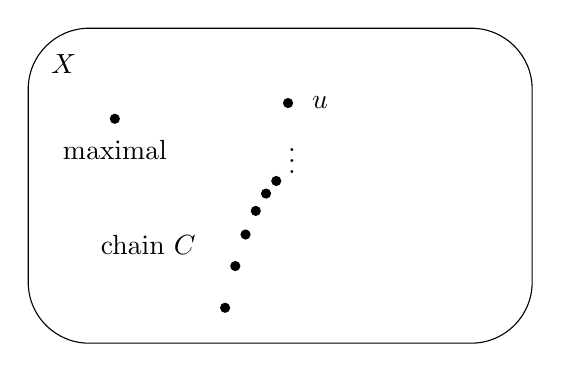
\begin{tikzpicture}[scale=1]
    \tikzstyle{v}=[circle, fill=black, inner sep=1.3pt]
    \draw[rounded corners=22pt] (-3.2,-1.7) rectangle (3.2,2.3);
    \node at (-2.75,1.85) {$X$};
    \foreach \i/\y in {0/-1.25, 1/-0.72, 2/-0.32, 3/-0.02, 4/0.2, 5/0.36} {
      \node[v] at ({-0.7 + 0.13*\i}, \y) {};
    }
    \node at (0.15,0.72) {$\vdots$};
    \node[left] at (-0.95,-0.45) {chain $C$};
    \node[v] at (0.1,1.35) {};
    \node[right] at (0.28,1.35) {$u$};
    \node[v] at (-2.1,1.15) {};
    \node[below] at (-2.1,1.0) {maximal};
  \end{tikzpicture}
\end{center}

\begin{proof}
  Suppose $X$ has no maximal element. Then for each $x \in X$ we may choose $x' \in X$ with $x' > x$, and for each chain $C$ we may choose an upper bound $u(C)$; both of these use the axiom of choice.

  Let $\gamma = \gamma(X)$ be the Hartogs' ordinal of $X$ from Theorem~\ref{thm:hartogs}. Pick any $x \in X$ and define $x_\alpha$ for $\alpha < \gamma$ by transfinite recursion:
  \begin{align*}
    x_0 &= x, \\
    x_{\alpha^+} &= (x_{\alpha})', \\
    x_{\lambda} &= u(\{x_\alpha \mid \alpha < \lambda\}) \quad \text{for } \lambda \text{ a non-zero limit.}
  \end{align*}
  For this to make sense we need $\{x_\alpha \mid \alpha < \lambda\}$ to be a chain, which follows by induction: at each stage we only ever add an element above everything so far.

  But then $\alpha \mapsto x_\alpha$ is strictly increasing, hence injective, so we have injected $\gamma$ into $X$, contradicting the definition of $\gamma(X)$.
\end{proof}

The proof is short, but it should not be mistaken for an easy one: it rests on the whole apparatus of well-orderings, transfinite recursion, ordinals and Hartogs' lemma. The axiom of choice is used only in the very first line.

\begin{example}[The Hypothesis of Zorn's Lemma]~
  \begin{enumerate}[label=(\roman*)]
    \item In $\mathcal{P}(S)$ under inclusion, every chain has an upper bound (its union), and indeed there is a maximal element, namely $S$.
    \item In the poset of \emph{finite} subsets of an infinite $S$, the chain $\{1\} \subseteq \{1,2\} \subseteq \cdots$ has no upper bound, and there is no maximal element.
    \item In $[0,1)$ with the usual order, every chain has an upper bound in $[0,1]$ but not always in $[0,1)$, and there is no maximal element. This shows how carefully the upper bound must be checked to lie in the poset itself -- it is the step that fails most often in practice.
  \end{enumerate}
\end{example}

\subsection{Applications of Zorn's Lemma}\label{sec:zornapps}

Proofs using Zorn's lemma nearly always look the same. We choose a poset whose elements are `partial solutions' to our problem, usually a family of subsets ordered by inclusion; we check that the union of a chain of partial solutions is a partial solution; and then we check that a maximal partial solution is a solution.

\begin{theorem}[Every Vector Space has a Basis]
  Every vector space $V$ has a basis.
\end{theorem}
\begin{proof}
  Let $X$ be the set of all linearly independent subsets of $V$, ordered by inclusion. Note $X \neq \emptyset$ as $\emptyset \in X$.

  We claim a maximal element $A$ of $X$ is a basis. It is linearly independent by definition, and if it did not span then there would be some $v \in V$ outside its span, and $A \cup \{v\}$ would be linearly independent, contradicting maximality.

  So we apply Zorn's lemma. Let $\{A_i \mid i \in I\}$ be a chain in $X$ and let $A = \bigcup_{i \in I} A_i$. Then $A \supseteq A_i$ for all $i$, so we need only check $A \in X$, i.e.\ that $A$ is linearly independent. Suppose we had a linear dependence $\lambda_1 x_1+\cdots+\lambda_n x_n=0$ with $x_1, \ldots, x_n \in A$ and the $\lambda_i$ not all zero. Each $x_j$ lies in some $A_{i_j}$, and since the $A_i$ form a chain, one of $A_{i_1}, \dots, A_{i_n}$ contains all the others, and hence contains all of $x_1, \dots, x_n$. That contradicts its linear independence.
\end{proof}

Observe that linear algebra was used only at the very last step, to see that a maximal element does the job. This is typical. Note also that the theorem is highly non-constructive: it tells us that $\R$ has a basis as a vector space over $\Q$ (a \emph{Hamel basis}), but no such basis can be written down.

\begin{theorem}[Every Ring has a Maximal Ideal]
  Let $R$ be a non-trivial ring with $1$. Then $R$ has a maximal ideal.
\end{theorem}
\begin{proof}
  Let $X$ be the set of proper ideals of $R$, ordered by inclusion; it is non-empty as $\{0\} \in X$. Given a non-empty chain $\{I_j \mid j \in J\}$ in $X$, the union $I = \bigcup_j I_j$ is an ideal (any two elements of $I$ lie in a common $I_j$, so $I$ is closed under addition, and it is clearly closed under multiplication by $R$), and it is proper, since $1 \notin I_j$ for any $j$ and so $1 \notin I$. So $I$ is an upper bound in $X$. By Zorn's lemma $X$ has a maximal element, which is by definition a maximal ideal.
\end{proof}

A third application, this time with no algebra in sight at all.

\begin{theorem}[Order-Extension Principle]
  Every partial order $(X, \leq)$ can be extended to a total order on $X$; that is, there is a total order $\preceq$ on $X$ with $x \leq y$ implying $x \preceq y$.
\end{theorem}
\begin{proof}
  Regard a partial order on $X$ as a subset of $X \times X$, and let $P$ be the set of all partial orders on $X$ containing $\leq$, ordered by inclusion. It is non-empty as $\leq \, \in P$.

  Given a non-empty chain in $P$, its union is again a partial order: reflexivity is clear, and given two or three pairs in the union we may find a single member of the chain containing all of them, in which transitivity and antisymmetry hold. So it is an upper bound, and Zorn's lemma gives a maximal $\preceq \, \in P$.

  Finally, $\preceq$ is total. If $x$ and $y$ were incomparable, consider
  $$R = \; \preceq \cup \; \{(a, b) \mid a \preceq x \text{ and } y \preceq b\}.$$
  One checks that $R$ is a partial order (transitivity is a short case-check, and antisymmetry uses the incomparability of $x$ and $y$) which strictly contains $\preceq$, contradicting maximality.
\end{proof}

We can also use Zorn to dispense with the countability assumption in our discussion of propositional logic, where we needed to enumerate $L$.

\begin{theorem}[Model Existence Lemma, Uncountable Case]\label{thm:propmodelexistenceuncountable}
  Let $P$ be any set of primitive propositions and let $S \subseteq L(P)$ be consistent. Then $S$ has a model.
\end{theorem}
\begin{proof}
  As in the proof of Theorem~\ref{thm:propmodelexistence}, it is enough to find a consistent $\overline S \supseteq S$ such that for every $t \in L$, either $t \in \overline S$ or $\lnot t \in \overline S$; the valuation $v(t) = \ii[t \in \overline S]$ then works verbatim.

  We claim that a \emph{maximal} consistent $\overline S \supseteq S$ has this property. Indeed if $t \notin \overline S$, then $\overline S \cup \{t\}$ is inconsistent by maximality, so $\overline S \cup \{t\} \vdash \bot$, so $\overline S \vdash \lnot t$ by the deduction theorem. Then $\overline S \cup \{\lnot t\}$ is consistent (anything it proves, $\overline S$ already proves), so $\lnot t \in \overline S$ by maximality again.

  So we must show a maximal consistent extension exists. Let $X = \{T \subseteq L \mid T \supseteq S, \, T \text{ consistent}\}$, ordered by inclusion, which is non-empty as $S \in X$. Let $\{T_i \mid i \in I\}$ be a non-empty chain in $X$ and let $T = \bigcup_i T_i$. Certainly $T \supseteq S$. To see $T$ is consistent, suppose $T \vdash \bot$. As proofs are finite, there are $t_1, \dots, t_n \in T$ with $\{t_1, \dots, t_n\} \vdash \bot$, and as the $T_i$ are nested, some $T_k$ contains all of the $t_j$ -- making $T_k$ inconsistent, a contradiction. So $T \in X$ is an upper bound for the chain, and Zorn's lemma provides a maximal element of $X$.
\end{proof}

\subsection{The Well-Ordering Principle}

Zorn's lemma also delivers the result promised in Section~\ref{sec:ordarith}, that every set can be well-ordered -- including $\R$, for which no explicit well-ordering can be described.

\begin{theorem}[Well-Ordering Principle]\label{thm:wop}
  Assume Zorn's lemma. Then every set $S$ can be well-ordered.
\end{theorem}
\begin{proof}
  Let $X$ be the set of pairs $(A, R)$ where $A \subseteq S$ and $R$ is a well-ordering of $A$, ordered by $(A, R) \leq (A', R')$ if $(A', R')$ extends $(A, R)$ -- that is, $A$ is an initial segment of $A'$ and $R'$ agrees with $R$ on $A$. Note $X \neq \emptyset$ as $(\emptyset, \emptyset) \in X$.

  Given a non-empty chain $\{(A_i, R_i) \mid i \in I\}$ in $X$, the family $\{A_i\}$ is nested, so by Proposition~\ref{prop:nestedunion} the pair $(\bigcup_i A_i, \bigcup_i R_i)$ is a well-ordering, and it clearly extends each $(A_i, R_i)$. So it is an upper bound.

  By Zorn's lemma there is a maximal $(A, R) \in X$. If $A \neq S$ we may take $x \in S \setminus A$ and well-order $A \cup \{x\}$ by making $x$ greater than everything in $A$; this extends $(A, R)$ strictly, contradicting maximality. So $A = S$.
\end{proof}

\subsection{Zorn's Lemma and the Axiom of Choice}

We assumed the axiom of choice to prove Zorn's lemma, and Zorn's lemma to prove the well-ordering principle. The circle closes with the following.

\begin{theorem}[The Axiom of Choice]
  Assume the well-ordering principle. Then for any family $\{A_i \mid i \in I\}$ of non-empty sets there is a \vocab{choice function} $f: I \rightarrow \bigcup_{i \in I} A_i$ with $f(i) \in A_i$ for all $i$.
\end{theorem}
\begin{proof}
  Well-order $\bigcup_{i \in I} A_i$, and define $f(i)$ to be the least element of $A_i$.
\end{proof}

So the axiom of choice, Zorn's lemma and the well-ordering principle are all equivalent, over the other axioms of set theory. It is worth remarking on where choice was really needed: making \emph{one} arbitrary choice is not an axiom at all -- a set being non-empty means precisely that it has an element -- and by induction, finitely many choices are also free. It is only the passage to infinitely many simultaneous arbitrary choices that requires an axiom.

The axiom of choice is unlike the other axioms in that the object it produces is not determined by its inputs: the union of $A$ and $B$ is a specific set, whereas a choice function for the family $\{1, 2\}$ could be either of two things. This is why proofs using it are non-constructive. That said, plenty of proofs that do not use choice are also non-constructive, so this should not be overstated.

\subsection{The Bourbaki--Witt Theorem}

We close the section with a result in the same family as Zorn's lemma, but which needs no choice at all. Call a poset $X$ \vocab{chain-complete} if every non-empty chain in $X$ has a supremum.

\begin{theorem}[Bourbaki--Witt]
  Let $X$ be a non-empty chain-complete poset and let $f: X \to X$ be \emph{inflationary}, meaning $f(x) \geq x$ for all $x$. Then $f$ has a fixed point.
\end{theorem}

Given Zorn's lemma this is immediate: a chain-complete poset satisfies the hypotheses of Zorn (a non-empty chain has its supremum as an upper bound, and the empty chain has any element of the non-empty $X$), so $X$ has a maximal element $x$, and then $f(x) \geq x$ forces $f(x) = x$. What is interesting is that no choice is required.

\begin{proof}[Proof without choice]
  Fix $x_0 \in X$ and let $Y \subseteq X$ be the least subset with $x_0 \in Y$ that is closed under $f$ and under suprema of non-empty chains (namely, the intersection of all such subsets). One checks by induction on this closure that $Y$ is itself a chain: the point is that $f$ and suprema are the only ways to produce new elements, and neither can create incomparability, though verifying this carefully takes some work.

  Granting that $Y$ is a chain, it has a supremum $s = \sup Y \in Y$. Then $f(s) \in Y$, so $f(s) \leq s$, while $f(s) \geq s$ as $f$ is inflationary. So $f(s) = s$.
\end{proof}

The contrast with Zorn's lemma is instructive: there we had to \emph{choose} some $x' > x$ at each stage, and it is exactly that choice which the axiom of choice supplies. Here the function $f$ tells us what to do next, so there is nothing to choose.

\section{Predicate Logic}\label{sec:predicate}

Propositional logic cannot express any of the statements we actually care about, because it has no way of talking about \emph{objects}. We now upgrade to predicate logic, also called \emph{first-order logic}, in which we may quantify over the elements of a structure. Everything from Section 1 will reappear -- a language, valuations (now structures), axioms, proofs, soundness, completeness, compactness -- but each with more moving parts.

\subsection{Languages}

\begin{definition}[Language]
  Let $\Omega$ (the \vocab{function symbols}) and $\Pi$ (the \vocab{relation symbols}) be disjoint sets, and let $\alpha: \Omega \cup \Pi \rightarrow \N$ be a function, called the \vocab{arity}.

  The \vocab{language} $L = L(\Omega, \Pi, \alpha)$ is the set of formulae, defined as follows.
  \begin{itemize}
    \item \emph{Variables.} We have variables $x_1, x_2, \dots$ (also written $x, y, z, \dots$).
    \item \emph{Terms.} These are defined inductively by
    \begin{enumerate}[label=(\roman*)]
      \item every variable is a term;
      \item if $f \in \Omega$ with $\alpha(f) = n$, and $t_1, \dots, t_n$ are terms, then $f(t_1, \dots, t_n)$ is a term.
    \end{enumerate}
    \item \emph{Atomic formulae.} There are three sorts:
    \begin{enumerate}[label=(\roman*)]
      \item $\bot$;
      \item $(s = t)$ for any terms $s, t$;
      \item $\phi(t_1, \dots, t_n)$ for any $\phi \in \Pi$ with $\alpha(\phi) = n$ and terms $t_1, \dots, t_n$.
    \end{enumerate}
    \item \emph{Formulae.} These are defined inductively by
    \begin{enumerate}[label=(\roman*)]
      \item atomic formulae are formulae;
      \item $(p \Rightarrow q)$ is a formula for any formulae $p, q$;
      \item $(\forall x) p$ is a formula for any formula $p$ and variable $x$.
    \end{enumerate}
  \end{itemize}
\end{definition}

A function symbol of arity $0$ is a \vocab{constant}. As before, we use the abbreviations $\lnot$, $\land$, $\lor$, and we write $(\exists x) p$ for $\lnot (\forall x)(\lnot p)$.

\begin{example}[The Language of Groups]
  Take $\Omega = \{m, i, e\}$ and $\Pi = \emptyset$, with $\alpha(m) = 2$, $\alpha(i) = 1$ and $\alpha(e) = 0$. Then $e$, $x_1$, $m(x_1, x_2)$ and $i(m(x_1,x_1))$ are terms, and $(m(e, e) = e)$ and $(\forall x)(m(x, i(x)) = e)$ are formulae. The theory of groups is the set consisting of the associativity axiom, the identity axioms and the inverse axioms, written out in this language.
\end{example}

\begin{example}[Other Languages]
  For posets, take $\Omega = \emptyset$ and $\Pi = \{\leq\}$ with $\alpha(\leq) = 2$. For fields, take $\Omega = \{+, \cdot, -, 0, 1\}$ with the evident arities and $\Pi = \emptyset$. For graphs, take $\Omega = \emptyset$ and $\Pi = \{\sim\}$ with $\alpha(\sim) = 2$.
\end{example}

It cannot be stressed enough that a formula is at this stage a string of meaningless symbols; it makes no sense to ask whether it is true. In particular the symbols in $\Omega$ and $\Pi$ carry no meaning beyond their arity.

\begin{definition}[Closed Term]
  A term is \vocab{closed} if it contains no variables.
\end{definition}

\begin{definition}[Free and Bound Variables]
  An occurrence of a variable $x$ in a formula $p$ is \vocab{bound} if it lies inside the brackets of a quantifier $(\forall x)$, and \vocab{free} otherwise.
\end{definition}

\begin{definition}[Sentence]
  A \vocab{sentence} is a formula with no free variables.
\end{definition}

For instance, in the language of groups $(\forall x)(m(x, y) = e)$ has $x$ bound and $y$ free, so it is not a sentence; it says something only once we know what $y$ is.

\begin{definition}[Substitution]
  For a formula $p$, a variable $x$ and a term $t$, the \vocab{substitution} $p[t/x]$ is the formula obtained by replacing each free occurrence of $x$ in $p$ by $t$.
\end{definition}

\subsection{Semantic Entailment}

In propositional logic we interpreted the language in $\{0, 1\}$ using valuations. Now we must interpret it in a set carrying operations and relations of the right arities.

\begin{definition}[Structure]
  An \vocab{$L$-structure} is a non-empty set $A$ together with a function $f_A: A^n \rightarrow A$ for each $f \in \Omega$ with $\alpha(f) = n$, and a relation $\phi_A \subseteq A^n$ for each $\phi \in \Pi$ with $\alpha(\phi) = n$.
\end{definition}

\begin{remark}
  We explicitly forbid $A$ from being empty, which makes life much easier later on (in an empty structure $(\forall x)p$ would hold vacuously for every $p$, including $p = \bot$).
\end{remark}

\begin{example}
  In the language of groups, an $L$-structure is a set with a binary operation, a unary operation and a distinguished element -- no axioms required. Every group is an $L$-structure, but so is $\N$ with $m(x,y) = x + y$, $i(x) = x$ and $e = 0$.
\end{example}

We now define what it means for a sentence to hold in a structure. The definition is a mouthful, but after it is made we can largely forget it.

\begin{definition}[Interpretation]
  For each sentence $p$ and $L$-structure $A$, the \vocab{interpretation} $p_A \in \{0, 1\}$ is defined inductively as follows.
  \begin{itemize}
    \item \emph{Closed terms.} Define $t_A \in A$ for each closed term $t$ by
    $$
    (f(t_1, \dots, t_n))_A = f_A((t_1)_A, \dots, (t_n)_A)
    $$
    for $f \in \Omega$ with $\alpha(f) = n$ and $t_1, \dots, t_n$ closed terms.
    \item \emph{Atomic formulae.} We take
    \begin{align*}
      \bot_A &= 0,\\
      (s = t)_A &= \ii[s_A = t_A],\\
      (\phi(t_1, \dots, t_n))_A &= \ii[((t_1)_A, \dots, (t_n)_A) \in \phi_A].
    \end{align*}
    \item \emph{Sentences.} We take
    \begin{align*}
      (p \Rightarrow q)_A &= \ii[\text{not } (p_A = 1 \text{ and } q_A = 0)], \\
      ((\forall x)p)_A &= \ii[\,p[\overline{a}/x]_{\overline{A}} = 1 \text{ for all } a\in A\,],
    \end{align*}
    where for $a \in A$ we form a new language $L'$ by adding a constant $\overline{a}$, and make $A$ into an $L'$-structure $\overline{A}$ by setting $\overline{a}_{\overline{A}} = a$.
  \end{itemize}
\end{definition}

The last clause is the only awkward one, and the awkwardness is unavoidable: to say that $(\forall x) p$ holds we must talk about $p$ with $x$ replaced by an \emph{element} of $A$, and elements of $A$ are not symbols of the language until we make them so.

\begin{definition}[Theory]
  A \vocab{theory} is a set of sentences.
\end{definition}

\begin{definition}[Model]
  If $p_A = 1$ we say $p$ \vocab{holds} in $A$, or is \vocab{true} in $A$, or that $A$ is a \vocab{model} of $p$. For a theory $S$, a model of $S$ is a structure which is a model of every $s \in S$.
\end{definition}

\begin{definition}[Semantic Entailment]
  For a theory $S$ and a sentence $t$, we say $S$ \vocab{entails} $t$, written $S \models t$, if every model of $S$ is a model of $t$. We call $t$ a \vocab{tautology}, written $\models t$, if $\emptyset \models t$.
\end{definition}

The word \emph{first-order} refers to the fact that our variables range over \emph{elements} of the structure, not over subsets of it. This restriction is what makes the theory work, and also what makes it weak, as we will see.

\subsection{Syntactic Implication}

As before we need axioms and deduction rules. We keep the three propositional axioms and add two describing equality and two describing $\forall$.

\begin{axiom}[Axioms of Predicate Logic]~
  \begin{enumerate}[label=(\arabic*)]
    \item $p \Rightarrow (q \Rightarrow p)$ for any formulae $p, q$;
    \item $[p \Rightarrow (q \Rightarrow r)] \Rightarrow [(p \Rightarrow q) \Rightarrow (p \Rightarrow r)]$ for any formulae $p, q, r$;
    \item $(\lnot \lnot p) \Rightarrow p$ for any formula $p$;
    \item $(\forall x)(x = x)$ for any variable $x$;
    \item $(\forall x)(\forall y)[(x = y) \Rightarrow (p \Rightarrow p[y/x])]$ for any variables $x, y$ and formula $p$ with $y$ not occurring bound in $p$;
    \item $[(\forall x)p] \Rightarrow p[t/x]$ for any formula $p$, variable $x$ and term $t$, with no free variable of $t$ occurring bound in $p$;
    \item $[(\forall x)(p\Rightarrow q)] \Rightarrow [p\Rightarrow(\forall x)q]$ for any formulae $p, q$ with $x$ not occurring free in $p$.
  \end{enumerate}
\end{axiom}

The side conditions in (5), (6) and (7) all guard against accidental capture of variables. For example, without the condition in (6), taking $p$ to be $(\exists y)(x \neq y)$ and $t$ to be $y$ would let us deduce the false statement $(\exists y)(y \neq y)$ from the true statement $(\forall x)(\exists y)(x \neq y)$.

\begin{definition}[Deduction Rules]
  The \vocab{deduction rules} are
  \begin{enumerate}[label=(\roman*)]
    \item \emph{modus ponens}: from $p$ and $p \Rightarrow q$ we may deduce $q$;
    \item \emph{generalisation}: from $p$ we may deduce $(\forall x)p$, provided that no premise used in the proof of $p$ so far has $x$ as a free variable.
  \end{enumerate}
\end{definition}

The proviso on generalisation is essential: from the premise `$x$ is even' we must not be allowed to deduce that everything is even.

\begin{definition}[Proof and Syntactic Implication]
  A \vocab{proof} of $p$ from $S$ is a finite sequence of formulae, each of which is an axiom, or a member of $S$, or obtained from earlier lines by modus ponens or generalisation, and whose last line is $p$. If such a proof exists we write $S \vdash p$, and say $S$ \vocab{proves} $p$. If $\emptyset \vdash p$ we call $p$ a \vocab{theorem}.
\end{definition}

As in the propositional case we say $S$ is \vocab{consistent} if $S \not\vdash \bot$.

\begin{example}[A Proof in Predicate Logic]
  We show $\vdash [(\forall x)p] \Rightarrow (\exists x)p$, that is, $\vdash [(\forall x)p] \Rightarrow \lnot(\forall x)(\lnot p)$. By the deduction theorem it is enough to show
  $$\{(\forall x)p, \; (\forall x)(\lnot p)\} \vdash \bot.$$
  From $(\forall x) p$ and axiom (6) with $t = x$ we get $p$; from $(\forall x)(\lnot p)$ and axiom (6) we get $\lnot p$, that is, $p \Rightarrow \bot$; and modus ponens gives $\bot$. Note where non-emptiness of structures is hiding: semantically, $[(\forall x)p] \Rightarrow (\exists x)p$ would fail in an empty structure.
\end{example}

\begin{example}[Why Generalisation Needs its Proviso]
  Without the proviso we could argue: from the premise $p(x)$ (`$x$ is even'), deduce $(\forall x)\,p(x)$. But $\{p(x)\} \not\models (\forall x)p(x)$, as we see by taking the structure $\N$ with $p$ interpreted as `is even': the premise holds for some elements and the conclusion for none. Soundness would fail immediately.
\end{example}

\subsection{The Deduction Theorem}

\begin{proposition}[Deduction Theorem]\label{prop:preddeduction}
  Let $S$ be a set of formulae and $p, q$ formulae. Then $S \vdash (p \Rightarrow q)$ if and only if $S \cup \{p\} \vdash q$.
\end{proposition}
\begin{proof}
  The proof is exactly that of Theorem~\ref{thm:deduction}, except that in the backwards direction we must also handle lines obtained by generalisation.

  So suppose the line $(\forall x) r$ was obtained from an earlier line $r$ by generalisation, and by induction we have a proof of $p \Rightarrow r$ from $S$; we want $S \vdash p \Rightarrow (\forall x) r$.

  By the condition on generalisation, no premise used in the proof of $r$ from $S \cup \{p\}$ has $x$ free. Hence no premise used in our proof of $p \Rightarrow r$ from $S$ has $x$ free, so we may apply generalisation to get $S \vdash (\forall x)(p \Rightarrow r)$.

  If $x$ is not free in $p$, axiom (7) and modus ponens give $S \vdash p \Rightarrow (\forall x) r$ as required. If $x$ \emph{is} free in $p$, then $p$ was not among the premises used in the proof of $r$ from $S \cup \{p\}$, so in fact $S \vdash r$; then generalisation gives $S \vdash (\forall x) r$, and axiom (1) gives $S \vdash p \Rightarrow (\forall x) r$.
\end{proof}

\subsection{Soundness}

\begin{proposition}[Soundness]
  Let $S$ be a theory and $p$ a sentence. Then $S \vdash p$ implies $S \models p$.
\end{proposition}
\begin{proof}
  Let $A$ be a model of $S$ and let $t_1, \dots, t_n = p$ be a proof of $p$ from $S$. As in the propositional case we check by induction that each $t_i$ holds in $A$ -- interpreting a formula with free variables as its universal closure. Each axiom holds in every structure (this is a routine but tedious check, one case per axiom), members of $S$ hold as $A \models S$, and each of the two deduction rules preserves holding in $A$: modus ponens by the definition of $(p \Rightarrow q)_A$, and generalisation by the definition of $((\forall x)p)_A$ together with the proviso.
\end{proof}

\subsection{The Model Existence Lemma}

The interesting direction, as before, is adequacy, and again it reduces to the statement that a consistent theory has a model. But now we have to build an entire structure out of nothing, and the only raw material available is the language itself.

Before the proof, here are the four ideas that go into it, since the proof is otherwise unmotivated.

\begin{enumerate}[label=(\roman*)]
  \item \emph{Build the model out of the language.} Take the underlying set to be the set of closed terms of $L$, with each function symbol acting in the obvious way: $f([t_1], \dots, [t_n]) = [f(t_1, \dots, t_n)]$.
  \item \emph{Quotient.} If $S$ is the theory of fields, then $S \vdash (1 + 0 = 1)$, but `$1+0$' and `$1$' are different strings. So we quotient the closed terms by $s \sim t$ if $S \vdash (s = t)$.
  \item \emph{Make $S$ complete.} Let $S$ be the field axioms together with the sentence $(1+1 = 0) \lor (1+1+1 = 0)$. Then $S$ proves neither disjunct, so in our quotient $[1+1] \neq [0]$ and $[1+1+1] \neq [0]$, and the structure we build is a field of neither characteristic $2$ nor $3$ -- so not a model. We fix this by extending $S$ to a \emph{maximal} consistent theory, using Zorn's lemma exactly as in Theorem~\ref{thm:propmodelexistenceuncountable}.
  \item \emph{Add witnesses.} Let $S$ be the field axioms together with $(\exists x)(x \cdot x = 1+1)$. There need be no closed term $t$ with $[t \cdot t] = [1+1]$, so again our structure fails. We fix this by adding, for each sentence $(\exists x)p$ in our theory, a brand new constant $c$ to the language and the sentence $p[c/x]$ to the theory.
\end{enumerate}
Unfortunately (iv) enlarges the language, which may destroy the maximality won in (iii), so we must alternate between the two infinitely often and take the union.

\begin{theorem}[Model Existence Lemma]\label{thm:predmodelexistence}
  Every consistent theory has a model.
\end{theorem}
\begin{proof}
  Let $S$ be consistent in the language $L = L(\Omega, \Pi)$.

  \emph{Step 1: the theory.} Extend $S$ to a maximal consistent theory $S_1$ in $L$, using Zorn's lemma as in Theorem~\ref{thm:propmodelexistenceuncountable}. Such a theory is \vocab{complete}: for every sentence $p$, either $p \in S_1$ or $\lnot p \in S_1$. Now add witnesses: for each sentence $(\exists x) p \in S_1$ introduce a new constant $c_{(\exists x)p}$, let $C_1$ be the set of these, and let
  $$T_1 = S_1 \cup \{p[c_{(\exists x)p}/x] \mid (\exists x)p \in S_1\}$$
  in the language $L_1 = L(\Omega \cup C_1, \Pi)$. Then $T_1$ is consistent: a proof of $\bot$ from $T_1$ uses finitely many of the new sentences, and replacing each new constant throughout the proof by a fresh variable and using $(\exists x)p \in S_1$ finitely many times converts it into a proof of $\bot$ from $S_1$.

  Repeat: extend $T_1$ to a maximal consistent $S_2$ in $L_1$, add witnesses to get $T_2$ in $L_2$, and so on. Let $\overline{S} = \bigcup_{n \geq 1} S_n$ in the language $\overline{L} = L(\Omega \cup \bigcup_n C_n, \Pi)$.

  We claim $\overline S$ is consistent, complete and has witnesses. It is consistent since a proof of $\bot$ from it is finite, so comes from some $S_n$. It is complete: a sentence $p$ of $\overline L$ is a finite string, so lies in some $L_n$, and $S_{n+1}$ is complete in $L_n$, so proves $p$ or $\lnot p$. And it has witnesses: if $(\exists x) p \in \overline S$ then $(\exists x)p \in S_n$ for some $n$, and $T_n$ supplied a witness.

  \emph{Step 2: the structure.} On the set of closed terms of $\overline L$ define $s \sim t$ if $\overline S \vdash (s = t)$. This is an equivalence relation, by axioms (4) and (5). Let $A$ be the set of equivalence classes, which is non-empty as $\overline L$ has at least one constant (if $\Omega$ had none, the witnesses supplied one -- and if $\overline S$ has no existential sentences at all we may add a constant by hand). Make $A$ into an $\overline L$-structure by
  \begin{align*}
    f_A([t_1], \dots, [t_n]) &= [f(t_1, \dots, t_n)], \\
    \phi_A &= \{([t_1], \dots, [t_n]) \mid \overline S \vdash \phi(t_1, \dots, t_n)\},
  \end{align*}
  both of which are well-defined by axiom (5).

  \emph{Step 3: $A$ is a model.} We claim that for every sentence $p$ of $\overline L$,
  $$p_A = 1 \iff \overline S \vdash p,$$
  which finishes the proof, since $S \subseteq \overline S$ so every $p \in S$ holds in $A$ (and $A$ is an $L$-structure by forgetting the new constants). We induct on the structure of $p$.

  If $p$ is $\bot$ then $\bot_A = 0$ and $\overline S \not\vdash \bot$. If $p$ is $(s = t)$ for closed terms $s, t$, then $\overline S \vdash (s=t)$ if and only if $[s] = [t]$ by the definition of $\sim$, if and only if $s_A = t_A$. Relations are the same by the definition of $\phi_A$.

  If $p$ is $(q \Rightarrow r)$, then since $\overline{S}$ is complete and consistent, $\overline S \vdash (q \Rightarrow r)$ if and only if $\overline S \vdash \lnot q$ or $\overline S \vdash r$. (If $\overline S \not\vdash \lnot q$ and $\overline S \not\vdash r$ then $\overline S \vdash q$ by completeness, so $\overline S \vdash r$ by modus ponens, a contradiction.) By induction this holds if and only if $q_A = 0$ or $r_A = 1$, which is the definition of $(q \Rightarrow r)_A = 1$.

  Finally consider $(\exists x)q$, which suffices since $(\forall x) q$ is $\lnot(\exists x)\lnot q$. If $\overline S \vdash (\exists x)q$ then $(\exists x) q \in \overline S$ by completeness, so there is a witness $c$ with $q[c/x] \in \overline S$, and by induction $q[c/x]_A = 1$, so $(\exists x)q$ holds in $A$. Conversely if $(\exists x) q$ holds in $A$, then since every element of $A$ is $[t]$ for some closed term $t$, we have $q[t/x]_A = 1$ for some closed term $t$, so $\overline S \vdash q[t/x]$ by induction, and hence $\overline S \vdash (\exists x)q$.
\end{proof}

\begin{corollary}[Adequacy]
  Let $S$ be a theory and $p$ a sentence. Then $S \models p$ implies $S \vdash p$.
\end{corollary}
\begin{proof}
  If $S \models p$ then $S \cup \{\lnot p\}$ has no model, so is inconsistent by Theorem~\ref{thm:predmodelexistence}. Then $S \cup \{\lnot p\} \vdash \bot$, so $S \vdash \lnot \lnot p$ by the deduction theorem, so $S \vdash p$ by axiom (3).
\end{proof}

\begin{theorem}[G\"odel's Completeness Theorem]
  Let $S$ be a theory and $p$ a sentence. Then $S \models p$ if and only if $S \vdash p$.
\end{theorem}
\begin{proof}
  Soundness and adequacy.
\end{proof}

\begin{remark}
  If $L$ is countable, Zorn's lemma is not needed above: we can enumerate the sentences and extend $S$ one at a time, as we did in the propositional case.
\end{remark}

Notice that there is no analogue of the decidability theorem here: to check $S \models p$ directly we would have to inspect every $L$-structure, of which there are a proper class. We will see in Section~\ref{sec:incompleteness} that this is not merely a failure of imagination.

\subsection{Compactness and the L\"owenheim--Skolem Theorems}

\begin{theorem}[Compactness Theorem]\label{thm:predcompactness}
  Let $S$ be a theory such that every finite subset of $S$ has a model. Then $S$ has a model.
\end{theorem}
\begin{proof}
  Replacing `has a model' by `is consistent' using the completeness theorem, this says that if every finite subset of $S$ is consistent then $S$ is consistent, which is immediate since proofs are finite.
\end{proof}

This has some startling consequences, all obtained by the same trick: write down a theory whose finite fragments are obviously satisfiable, and conclude that the whole thing is.

\begin{corollary}[Finiteness is Not First-Order]
  There is no theory $S$ in the language of groups whose models are precisely the finite groups.
\end{corollary}
\begin{proof}
  Suppose $S$ were such a theory. Let $\sigma_k$ be the sentence saying `there are at least $k$ elements', namely
  $$(\exists x_1)\cdots(\exists x_k)\Bigl(\bigwedge_{i < j} x_i \neq x_j\Bigr),$$
  and let $T = S \cup \{\sigma_k \mid k \in \N\}$. Any finite subset of $T$ mentions only finitely many $\sigma_k$, so has a model, namely a cyclic group of large enough order. By compactness $T$ has a model, which is a finite group with at least $k$ elements for every $k$ -- a contradiction.
\end{proof}

\begin{corollary}
  Let $S$ be a theory with arbitrarily large finite models. Then $S$ has an infinite model.
\end{corollary}
\begin{proof}
  Add the sentences $\sigma_k$ as above and apply compactness.
\end{proof}

\begin{corollary}[Connectedness is Not First-Order]
  There is no theory in the language of graphs whose models are precisely the connected graphs.
\end{corollary}
\begin{proof}
  Suppose $S$ were such a theory. Add two constants $a, b$ to the language and let
  $$T = S \cup \{\delta_k \mid k \in \N\},$$
  where $\delta_k$ is the sentence saying `there is no path from $a$ to $b$ of length $k$', which is a first-order sentence since it quantifies over the $k-1$ intermediate vertices. Any finite subset of $T$ mentions finitely many $\delta_k$, and has a model: take a long path, with $a$ and $b$ its endpoints. So by compactness $T$ has a model, which is a connected graph containing two vertices joined by no path at all -- a contradiction.
\end{proof}

\begin{theorem}[Upward L\"owenheim--Skolem]
  Let $S$ be a theory with an infinite model. Then $S$ has an uncountable model.
\end{theorem}
\begin{proof}
  Add constants $\{c_i \mid i \in I\}$ to $L$ for some uncountable set $I$, and let
  $$T = S \cup \{(c_i \neq c_j) \mid i, j \in I, \, i \neq j\}.$$
  Any finite $T' \subseteq T$ mentions only finitely many of the $c_i$, so an infinite model of $S$ is a model of $T'$ once we interpret those finitely many constants as distinct elements. By compactness $T$ has a model, which has at least $|I|$ elements.
\end{proof}

\begin{theorem}[Downward L\"owenheim--Skolem]
  Let $L$ be a countable language, that is, with $\Omega$ and $\Pi$ countable. Then if a theory $S$ in $L$ has a model, it has a countable model.
\end{theorem}
\begin{proof}
  If $S$ has a model then $S$ is consistent by soundness, and the model constructed in the proof of Theorem~\ref{thm:predmodelexistence} is countable: at each stage we add countably many constants to a countable language, and a countable union of countable sets is countable. So the set of closed terms, and hence its quotient, is countable.
\end{proof}

Putting these together gives \emph{Skolem's paradox}: the theory $\ZF$ of Section~\ref{sec:settheory} is written in a countable language, so if it has a model at all then it has a \emph{countable} model -- even though $\ZF$ proves the existence of uncountable sets. The resolution is that `uncountable' is interpreted inside the model: a set $x$ in the model is uncountable if the model contains no bijection between $x$ and $\omega$, and there is no reason for the model to contain every bijection that exists outside it.

\subsection{Categoricity}

Since a first-order theory can never pin down the size of its models, we may ask for the next best thing: that it pin down the model once the size is fixed.

\begin{definition}[Categoricity]
  A theory $S$ is \vocab{$\kappa$-categorical} if it has a model of cardinality $\kappa$ and any two such models are isomorphic.
\end{definition}

By the L\"owenheim--Skolem theorems, a theory with an infinite model has models of many different sizes, so no such theory can be categorical outright. But $\aleph_0$-categoricity does occur.

\begin{theorem}[Cantor]
  The theory of dense linear orders without endpoints is $\aleph_0$-categorical. In particular, every countable dense linear order without endpoints is isomorphic to $(\Q, <)$.
\end{theorem}
\begin{proof}[Proof sketch]
  Let $X = \{x_1, x_2, \dots\}$ and $Y = \{y_1, y_2, \dots\}$ be two such orders, enumerated (not in order!). We build an isomorphism by a \emph{back-and-forth} construction, extending a finite order-preserving partial map one point at a time, and alternating between the two sides so that every point gets used.

  At an odd stage we take the least-indexed $x$ not yet in the domain and find a partner for it in $Y$: the finitely many points already matched cut $Y$ into finitely many intervals, and we need a point of $Y$ in the interval corresponding to the position of $x$, which exists by density (or by the absence of endpoints, if $x$ lies beyond everything matched so far). At an even stage we do the same in reverse, taking the least-indexed $y$ not yet in the image.
  \begin{center}
    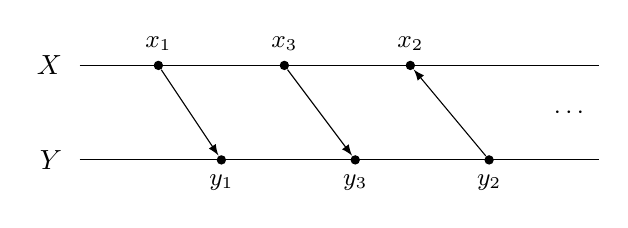
\begin{tikzpicture}[scale=1, >=latex]
      \tikzstyle{v}=[circle, fill=black, inner sep=1.2pt]
      \draw (-0.3,1.2) -- (6.3,1.2);
      \draw (-0.3,0) -- (6.3,0);
      \node[left] at (-0.4,1.2) {$X$};
      \node[left] at (-0.4,0) {$Y$};
      \node[v, label=above:{\small $x_1$}] (x1) at (0.7,1.2) {};
      \node[v, label=above:{\small $x_2$}] (x2) at (3.9,1.2) {};
      \node[v, label=above:{\small $x_3$}] (x3) at (2.3,1.2) {};
      \node[v, label=below:{\small $y_1$}] (y1) at (1.5,0) {};
      \node[v, label=below:{\small $y_2$}] (y2) at (4.9,0) {};
      \node[v, label=below:{\small $y_3$}] (y3) at (3.2,0) {};
      \draw[->] (x1) -- (y1);
      \draw[<-] (x2) -- (y2);
      \draw[->] (x3) -- (y3);
      \node[right] at (5.6,0.6) {\small $\cdots$};
    \end{tikzpicture}
  \end{center}
  Going forth at odd stages guarantees the map is defined everywhere; going back at even stages guarantees it is onto. The union of all these finite partial maps is therefore an isomorphism.
\end{proof}

Categoricity is useful because of the following test, which we state without proof: if a theory $S$ has no finite models and is $\kappa$-categorical for some infinite $\kappa$, then $S$ is \vocab{complete}, meaning that for every sentence $p$ either $S \vdash p$ or $S \vdash \lnot p$. So the theory of dense linear orders without endpoints is complete, and in particular any sentence true in $\Q$ is provable from those axioms. The theory of the next section is very far from having this property.

\subsection{Peano Arithmetic and Non-Standard Models}

Let us apply all this to arithmetic. Take $\Omega = \{0, s, +, \cdot\}$ with arities $0, 1, 2, 2$, and $\Pi = \emptyset$. Here $s$ is the successor function.

\begin{definition}[Peano Arithmetic]
  \vocab{Peano arithmetic}, written $\PA$, is the theory with axioms
  \begin{enumerate}[label=(\roman*)]
    \item $(\forall x)(s(x) \neq 0)$;
    \item $(\forall x)(\forall y)(s(x) = s(y) \Rightarrow x = y)$;
    \item $(\forall y_1)\cdots(\forall y_n)\bigl[\bigl(p[0/x] \land (\forall x)(p \Rightarrow p[s(x)/x])\bigr) \Rightarrow (\forall x)p\bigr]$ for each formula $p$ with free variables $x, y_1, \dots, y_n$;
    \item $(\forall x)(x + 0 = x)$;
    \item $(\forall x)(\forall y)(x + s(y) = s(x + y))$;
    \item $(\forall x)(x \cdot 0 = 0)$;
    \item $(\forall x)(\forall y)(x \cdot s(y) = x \cdot y + x)$.
  \end{enumerate}
\end{definition}

Axiom (iii) is the induction scheme, and the variables $y_i$ are called \emph{parameters}; without them we could not induct on a property like `$x \geq y$' with $y$ held fixed. Note that $\N$ is a model of $\PA$, so $\PA$ is consistent.

The crucial point is that (iii) is a scheme with one instance per \emph{formula}, and there are only countably many formulae. So $\PA$ asserts induction only for the countably many definable subsets of $\N$, and not for all of them. This is not a defect we can repair: a first-order language simply has no way to quantify over subsets.

The consequences are immediate. As $\PA$ has an infinite model, the upward L\"owenheim--Skolem theorem gives an uncountable model of $\PA$, which certainly is not isomorphic to $\N$. Such a model is called a \vocab{non-standard model of arithmetic}, and we can see what one looks like using compactness.

\begin{example}[A Non-Standard Model of Arithmetic]
  Add a constant $c$ to the language and let
  $$T = \PA \cup \{c \neq 0, \; c \neq s(0), \; c \neq s(s(0)), \; \dots\}.$$
  Any finite subset of $T$ has a model, namely $\N$ with $c$ interpreted as a large enough natural number. So by compactness $T$ has a model $A$. Inside $A$ the element $c$ is greater than every $s^n(0)$, so $A$ contains a copy of $\N$ followed by extra elements -- and since $A \models \PA$, every non-zero element has a predecessor, so those extra elements come in $\Z$-shaped blocks, ordered densely. Every theorem of $\PA$, and indeed every first-order sentence true in $\N$ that we care to add to $T$, holds in this strange structure too.
\end{example}

The same trick applied to the theory of ordered fields containing $\R$, with a constant $\varepsilon$ and the sentences $0 < \varepsilon < 1/n$ for all $n$, produces an ordered field containing $\R$ with a non-zero infinitesimal element -- a non-standard model of analysis, and the starting point for non-standard analysis.

Since the standard model $\N$ is not pinned down by $\PA$, one may ask which sentences $\PA$ does prove. The completeness theorem tells us that $\PA \vdash p$ if and only if $p$ holds in \emph{every} model, including the non-standard ones. So there is room for a sentence to be true in $\N$ but unprovable, and Section~\ref{sec:incompleteness} shows that there is one.

\section{Set Theory}\label{sec:settheory}

We have been using sets throughout, informally. We now write down axioms for them, in the first-order language of Section~\ref{sec:predicate}, and then see what the resulting universe looks like.

\subsection{The Axioms of ZF}

\begin{definition}[Zermelo--Fraenkel Set Theory]
  \vocab{Zermelo--Fraenkel set theory}, $\ZF$, is a first-order theory in the language with $\Omega = \emptyset$ and $\Pi = \{\in\}$, where $\alpha(\in) = 2$.
\end{definition}

A \emph{universe of sets} will mean a model of these axioms: a pair $(V, \in)$ where $V$ is a set and $\in$ is a binary relation on $V$ making the axioms true. Everything below is officially a statement of the form `let $(V, \in)$ be a model of $\ZF$; then \dots', or equivalently, by the completeness theorem, `$\ZF \vdash \dots$'.

\begin{axiom}[Extension]
  `Sets with the same members are equal':
  $$
  (\forall x)(\forall y)[(\forall z)(z \in x \Leftrightarrow z \in y) \Rightarrow x = y].
  $$
\end{axiom}

\begin{axiom}[Separation]
`For a set $x$ and a property $p$, we can form $\{z \in x \mid p(z)\}$':
$$
(\forall t_1)\cdots (\forall t_n) (\forall x)(\exists y)(\forall z)(z \in y \Leftrightarrow (z \in x \land p))
$$
for each formula $p$ with free variables $t_1, \dots, t_n, z$.
\end{axiom}

This is an axiom \emph{scheme}, with one instance per formula $p$. The parameters $t_i$ are needed to form sets such as $\{z \in x \mid z \in t\}$ for a variable $t$. Note carefully that we may only carve subsets out of a set we already have; the unrestricted version, allowing $\{z \mid p(z)\}$ for any $p$, is inconsistent by Russell's paradox, taking $p(z)$ to be $z \notin z$.

\begin{axiom}[Empty Set]
  `There is an empty set':
  $$
  (\exists x) (\forall y)(y \notin x).
  $$
  We write $\emptyset$ for this set, which is unique by extension.
\end{axiom}

\begin{axiom}[Pair Set]
  `We can form $\{x, y\}$':
  $$
(\forall x)(\forall y)(\exists z)(\forall t)(t \in z \Leftrightarrow (t = x \lor t = y)).
  $$
  We write $\{x, y\}$ for this $z$, and $\{x\}$ for $\{x, x\}$.
\end{axiom}

With pairs we can already encode ordered pairs and hence functions, entirely inside the language.

\begin{definition}[Ordered Pair]
  The \vocab{ordered pair} is $(x, y) = \{\{x\}, \{x, y\}\}$. One checks that $(x, y) = (z, t)$ if and only if $x = z$ and $y = t$, which is all we ever want from ordered pairs.
\end{definition}

\begin{definition}[Function]
  We say $f$ is a \vocab{function} if
  \begin{align*}
  &(\forall x)(x \in f \Rightarrow x \text{ is an ordered pair}) \\
  &\qquad \land \; (\forall x)(\forall y)(\forall z) [((x, y) \in f\land (x, z) \in f) \Rightarrow y = z],
  \end{align*}
  where `$x$ is an ordered pair' abbreviates $(\exists y)(\exists z)(x = (y,z))$. We say $x$ is the \vocab{domain} of $f$, written $x = \dom(f)$, if $f$ is a function and $(\forall y)(y \in x \Leftrightarrow (\exists z)((y, z) \in f))$. Then $f: x \rightarrow y$ abbreviates $(f\text{ is a function}) \land (x = \dom(f)) \land (\forall z)(\forall t)((z, t) \in f \Rightarrow t \in y)$.
\end{definition}

Back to the axioms.

\begin{axiom}[Union]
  `We can form unions':
  $$
(\forall x)(\exists y)(\forall z)(z \in y \Leftrightarrow (\exists t)(t \in x \land z \in t)).
  $$
  We write $y = \bigcup x$; note this is the union of the members of $x$, so that $A \cup B$ is $\bigcup\{A, B\}$.
\end{axiom}

Intersections need no axiom: $\bigcap x$ is a subset of any member of $x$, so separation provides it.

\begin{axiom}[Power Set]
  `We can form power sets':
  $$
  (\forall x)(\exists y)(\forall z)(z \in y \Leftrightarrow z \subseteq x),
  $$
  where $z \subseteq x$ abbreviates $(\forall t)(t \in z \Rightarrow t \in x)$. We write $\mathcal{P}(x)$ for this $y$.
\end{axiom}

\begin{axiom}[Infinity]
`There is an infinite set':
$$
(\exists x)(\emptyset \in x \land (\forall y)(y \in x \Rightarrow y^+ \in x)),
$$
where $y^+ = y \cup \{y\}$. A set satisfying this is called a \vocab{successor set}.
\end{axiom}

The intersection of all successor sets contained in a given one is again a successor set, so there is a least successor set; call it $\omega$. Its members are
$$\emptyset, \; \{\emptyset\}, \; \{\emptyset, \{\emptyset\}\}, \; \dots$$
which we name $0, 1, 2, \dots$, so that $n = \{0, 1, \dots, n-1\}$. Minimality of $\omega$ gives induction: if $x \subseteq \omega$ is a successor set then $x = \omega$, that is,
$$
(\forall x)[(x \subseteq \omega \land \emptyset \in x \land (\forall y)(y \in x \Rightarrow y^+ \in x)) \Rightarrow x = \omega].
$$
We can now define `$x$ is finite' to mean $(\exists y)(y \in \omega \land x \text{ bijects with } y)$, and `$x$ is countable' to mean `$x$ is finite or $x$ bijects with $\omega$'.

\begin{axiom}[Foundation]
  `Every non-empty set has an $\in$-minimal element':
  $$
  (\forall x)(x \neq \emptyset \Rightarrow(\exists y)(y \in x \land(\forall z)(z \in x \Rightarrow z \notin y))).
  $$
\end{axiom}

Foundation is the axiom that says sets are built up out of simpler sets: it forbids $x \in x$ (consider $\{x\}$) and infinite descending $\in$-chains. It plays for $\in$ exactly the role that the well-ordering condition played for $<$.

\begin{proposition}
  There is no set of all sets.
\end{proposition}
\begin{proof}
  Suppose $V$ were a set. Then by separation $R = \{x \in V \mid x \notin x\}$ is a set, and $R \in R$ if and only if $R \notin R$, a contradiction.
\end{proof}

So separation really is the correct restriction of the naive comprehension principle: it is strong enough for everything we do, and weak enough to survive Russell's argument. (In the presence of foundation we could argue differently, since then $x \notin x$ always, so $R = V$; but the proof above needs no such assumption.)

\subsection{A Digression on Classes}

One axiom remains, and to state it we need to be able to say things like `for each $i \in I$ we have a set $A_i$; now form $\{A_i \mid i \in I\}$'. The trouble is that the assignment $i \mapsto A_i$ may not be a function in $V$ -- it may be given by a formula rather than a set of ordered pairs.

\begin{definition}[Class]
  Let $(V, \in)$ be a model of $\ZF$. A \vocab{class} is a collection $C$ of points of $V$ such that, for some formula $p$ with free variable $x$ (and possibly parameters), we have $x \in C$ if and only if $p(x)$ holds.
\end{definition}

So classes are exactly the collections of the form $\{x \in V \mid p(x)\}$. Every set is a class, by separation. A class is a \vocab{proper class} if it is not a set, that is, if
$$\lnot (\exists y)(\forall x)(x \in y \Leftrightarrow p).$$
For example $V$ itself is a proper class, as is $\on$ by the Burali-Forti paradox. Statements about classes are always to be read as abbreviations for statements about the formulae defining them; classes are not objects of our theory.

\begin{definition}[Function-Class]
  A \vocab{function-class} $F$ is a collection of ordered pairs for which there is a formula $p$ with free variables $x, y$ (and possibly parameters) such that $(x, y) \in F$ if and only if $p$ holds, and such that $(x,y) \in F \land (x, z) \in F \Rightarrow y = z$.
\end{definition}

\begin{axiom}[Replacement]
  `The image of a set under a function-class is a set'. This is an axiom scheme, with an instance for each formula $p$:
  \begin{align*}
      & \underbrace{\left(\forall t_1\right) \ldots\left(\forall t_n\right)}_{\text {parameters }}\Bigl[\underbrace{(\forall x)(\forall y)(\forall z)(p \land p[z / y] \Rightarrow y=z)}_{p \text { is a function class }} \\
      & \qquad \Rightarrow (\forall x) \underbrace{(\exists y)(\forall z)(z \in y \Leftrightarrow(\exists t)(t \in x \land p[t / x , z / y]))}_{y \text { is the image of } x}\Bigr].
  \end{align*}
\end{axiom}

That completes the list: $\ZF$ consists of extension, separation, empty set, pair set, union, power set, infinity, foundation and replacement. Notice that we have not included the axiom of choice.

\begin{definition}[ZFC]
  \vocab{$\ZFC$} is $\ZF$ together with $\AC$, the axiom of choice, `every family of non-empty sets has a choice function':
  \begin{align*}
    (\forall f)\bigl[(\forall x)(x \in \dom f \Rightarrow f(x) \neq \emptyset) \Rightarrow \; &(\exists g)\bigl(\dom g = \dom f \\
    &\land \; (\forall x)(x \in \dom g \Rightarrow g(x) \in f(x))\bigr)\bigr],
  \end{align*}
  where a family of sets $\{A_i \mid i \in I\}$ is officially a function $f : I \to V$ with $f(i) = A_i$.
\end{definition}

\subsection{Transitive Sets}

We now start to investigate what $V$ must look like. The key notion is the following.

\begin{definition}[Transitive Set]
  A set $x$ is \vocab{transitive} if every member of a member of $x$ is a member of $x$:
  $$
  (\forall y)(\forall z)((y \in z \land z \in x) \Rightarrow y \in x).
  $$
\end{definition}

Equivalently, $y \in x$ implies $y \subseteq x$. For example $\emptyset$, $\{\emptyset\}$, $\{\emptyset, \{\emptyset\}\}$ and $\omega$ are transitive, whereas $\{\{\emptyset\}\}$ is not.

\begin{center}
  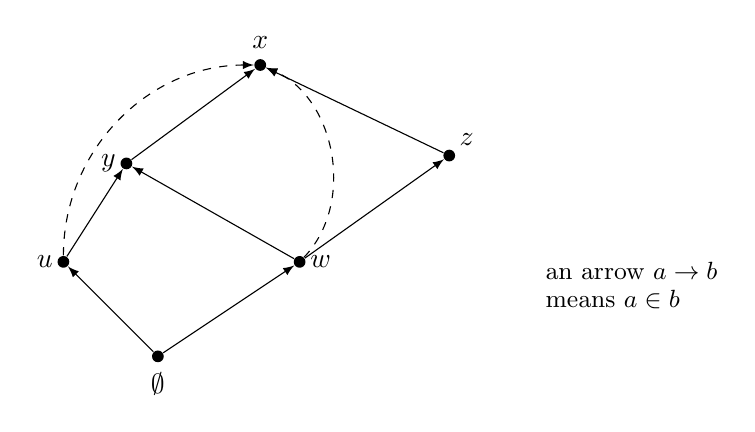
\begin{tikzpicture}[scale=1, >=latex]
    \tikzstyle{v}=[circle, fill=black, inner sep=1.5pt]
    \node[v, label=above:{$x$}] (x) at (0,2.5) {};
    \node[v, label={[label distance=-2pt]left:{$y$}}] (y) at (-1.7,1.25) {};
    \node[v, label={[label distance=-2pt]above right:{$z$}}] (z) at (2.4,1.35) {};
    \node[v, label={[label distance=-2pt]left:{$u$}}] (u) at (-2.5,0) {};
    \node[v, label={[label distance=-2pt]right:{$w$}}] (w) at (0.5,0) {};
    \node[v, label=below:{$\emptyset$}] (e) at (-1.3,-1.2) {};
    \draw[->] (y) -- (x); \draw[->] (z) -- (x);
    \draw[->] (u) -- (y); \draw[->] (w) -- (y); \draw[->] (w) -- (z);
    \draw[->] (e) -- (u); \draw[->] (e) -- (w);
    \draw[->, dashed] (u) to[bend left=45] (x);
    \draw[->, dashed] (w) to[bend right=55] (x);
    \node[right, align=left] at (3.5,-0.3) {\small an arrow $a \to b$\\[-2pt] \small means $a \in b$};
  \end{tikzpicture}
\end{center}

In the picture, the solid arrows are the memberships we started with, and $x$ is transitive precisely when all the dashed arrows are present as well. The other thing the picture shows is that following arrows downwards must terminate, which is exactly foundation, and this is what lets us do induction.

\begin{lemma}[Transitive Closure]\label{lem:transclosure}
  Every set $x$ is contained in a transitive set.
\end{lemma}
\begin{proof}
  We would like to form
  $$
  x \cup \left(\bigcup x\right)\cup \left(\bigcup \bigcup x\right)\cup \left(\bigcup\bigcup\bigcup x\right)\cup \cdots,
  $$
  which is clearly transitive and contains $x$. By the union axiom, it is enough to obtain the set $\{x, \bigcup x, \bigcup\bigcup x, \dots\}$, and for that it is enough by replacement to check that $n \mapsto \bigcup^n x$ is a function-class on $\omega$.

  Define `$f$ is an attempt' to mean
  \begin{align*}
    &(f \text{ is a function}) \land (\dom f \in \omega) \land (\dom f \neq \emptyset) \land (f(0) = x) \\
    &\qquad \land \; (\forall n)\bigl(n \in \dom f \land n \neq 0 \Rightarrow f(n) = \textstyle\bigcup f(n-1)\bigr).
  \end{align*}
  By the usual induction on $\omega$, any two attempts agree wherever both are defined, and for each $n \in \omega$ there is an attempt defined at $n$ (extend an attempt defined at $n - 1$ by one step, using the union and pair set axioms). So the formula
  $$p(y, z) = (\exists f)(f \text{ is an attempt} \land y \in \dom f \land f(y) = z)$$
  defines a function-class on $\omega$, and we are done.
\end{proof}

Since any intersection of transitive sets is transitive, it follows that $x$ is contained in a \emph{least} transitive set, called the \vocab{transitive closure} of $x$ and written $\TC(x)$.

\subsection{\texorpdfstring{$\in$}{Epsilon}-Induction and Foundation}

We want foundation to give us the principle: if $p(x)$ holds whenever $p(y)$ holds for all $y \in x$, then $p$ holds everywhere. This is $\in$-induction.

\begin{theorem}[Principle of $\in$-Induction]\label{thm:epsiloninduction}
  For each formula $p$ with free variables $t_1, \dots, t_n, x$,
  \begin{align*}
  \left(\forall t_1\right) \cdots\left(\forall t_n\right)\bigl[(\forall x)\bigl((\forall y)(y \in x \Rightarrow p(y)) \Rightarrow p(x)\bigr) \Rightarrow(\forall x)\,p(x)\bigr].
  \end{align*}
\end{theorem}
\begin{proof}
  Fix $t_1, \dots, t_n$ and suppose $\lnot(\forall x)\,p(x)$, so $\lnot p(x)$ for some $x$.

  We would like to choose an $\in$-minimal $x$ with $\lnot p(x)$ and apply the hypothesis, but $\{x \mid \lnot p(x)\}$ need not be a set. Instead let $t = \TC(\{x\})$ and $u = \{y \in t \mid \lnot p(y)\}$, which is a set by separation. Then $u \neq \emptyset$ as $x \in u$, so by foundation $u$ has an $\in$-minimal member $y$. Now $\lnot p(y)$; but if $z \in y$ then $z \in t$ by transitivity of $t$, and $z \notin u$ by minimality, so $p(z)$. So $p(z)$ holds for all $z \in y$, whence $p(y)$ by hypothesis, a contradiction.
\end{proof}

\begin{theorem}
  The axiom of foundation and the principle of $\in$-induction are equivalent, in the presence of the other axioms of $\ZF$.
\end{theorem}
\begin{proof}
  We have just derived $\in$-induction from foundation. Conversely, say that $x$ is \emph{regular} if
  $$(\forall y)(x \in y \Rightarrow y \text{ has an } \in\text{-minimal member}).$$
  Foundation says exactly that every $x$ is regular (given non-empty $y$, take $x \in y$). To prove this by $\in$-induction, it is enough to show that if every $y \in x$ is regular then $x$ is regular.

  So let $z$ be a set with $x \in z$. If $x$ is $\in$-minimal in $z$ we are done. Otherwise there is some $y \in x$ with $y \in z$; but $y$ is regular and $y \in z$, so $z$ has an $\in$-minimal member.
\end{proof}

\subsection{\texorpdfstring{$\in$}{Epsilon}-Recursion and Well-Founded Relations}

Having induction, we want recursion: to define $F(x)$ in terms of the values $F(y)$ for $y \in x$.

\begin{theorem}[$\in$-Recursion Theorem]\label{thm:epsilonrecursion}
Let $G$ be an everywhere-defined function-class. Then there is a unique everywhere-defined function-class $F$ such that
$$(\forall x)\bigl(F(x) = G(F|_x)\bigr),$$
where $F|_x = \{(y, F(y)) \mid y \in x\}$.
\end{theorem}
\begin{proof}
  Note first that $F|_x$ is a set by replacement, so the statement makes sense.

  Say `$f$ is an attempt' if
  \begin{align*}
    (f\text{ is a function}) \land (\dom f\text{ is transitive}) \land (\forall x)\bigl(x \in \dom f \Rightarrow f(x) = G(f|_x)\bigr),
  \end{align*}
  which makes sense as $\dom f$ is transitive, so $x \in \dom f$ gives $x \subseteq \dom f$.

  Any two attempts agree where both are defined, by $\in$-induction: if $f, f'$ agree at all $y \in x$ then $f|_x = f'|_x$, so $f(x) = G(f|_x) = G(f'|_x) = f'(x)$.

  For each $x$ there is an attempt defined at $x$, again by $\in$-induction. Indeed, suppose each $y \in x$ has an attempt defined at $y$; then for each such $y$ there is a unique attempt $f_y$ with domain $\TC(\{y\})$, and $\{f_y \mid y \in x\}$ is a set by replacement. Put $f = \bigcup\{f_y \mid y \in x\}$, a function by the previous paragraph, and then $f' = f \cup \{(x, G(f|_x))\}$ is an attempt defined at $x$.

  So we may define $F$ by the formula
  $$q(x, y) = (\exists f)(f \text{ is an attempt} \land x \in \dom f \land f(x) = y).$$
  Uniqueness of $F$ is another $\in$-induction.
\end{proof}

It is worth asking what properties of the relation $\in$ we actually used. There are two.
\begin{enumerate}[label=(\roman*)]
  \item It is \vocab{well-founded}: every non-empty set has an $\in$-minimal member.
  \item It is \vocab{local}: for each $y$, the collection $\{x \mid x \in y\}$ is a set, which is what let us build transitive closures.
\end{enumerate}
So for any well-founded, local relation given by a formula $r(x,y)$ we get $r$-induction and $r$-recursion by identical arguments. If $r$ is a relation on a \emph{set} $a$ then locality is automatic, so we only need $r$ to be well-founded. In particular, the induction and recursion theorems of Section 2 for well-orderings are special cases.

\subsection{Mostowski Collapse}

One result about well-orderings remains to be generalised, namely subset collapse. Its analogue answers the question: when can a relation on a set be modelled by $\in$?

\begin{definition}[Extensional Relation]
  A relation $r$ on a set $a$ is \vocab{extensional} if
  $$
  (\forall x, y \in a)\bigl[(\forall z \in a)(z \, r \, x \Leftrightarrow z \, r \, y) \Rightarrow x = y\bigr],
  $$
  that is, if it obeys the axiom of extension.
\end{definition}

\begin{theorem}[Mostowski Collapse Theorem]\label{thm:mostowski}
  Let $r$ be a well-founded extensional relation on a set $a$. Then there is a transitive set $b$ and a bijection $f: a \rightarrow b$ with
  $$(\forall x, y \in a)(x \, r \, y \Leftrightarrow f(x) \in f(y)).$$
  Moreover $b$ and $f$ are unique.
\end{theorem}
\begin{proof}
  Define $f$ by $r$-recursion on $a$ by
  $$f(x) = \{f(y) \mid y \, r \, x\},$$
  which is a set by replacement, and let $b = \{f(x) \mid x \in a\}$, again a set by replacement.

  Then $b$ is transitive by the definition of $f$ (any member of $f(x)$ is some $f(y)$, which is in $b$), and $f$ is surjective onto $b$ by the definition of $b$. So it remains to show $f$ is injective, and then $x \, r\, y \Leftrightarrow f(x) \in f(y)$ follows.

  We show $(\forall y \in a)(f(x) = f(y) \Rightarrow x = y)$ for each $x \in a$, by $r$-induction on $x$. So suppose the claim for all $t \, r \, x$, and let $y \in a$ with $f(x) = f(y)$. By the definition of $f$ we have $\{f(t) \mid t \, r\, x\} = \{f(u) \mid u \, r \, y\}$, so by the induction hypothesis $\{t \mid t \, r \, x\} = \{u \mid u\, r\, y\}$, and hence $x = y$ by extensionality.

  For uniqueness, if $f, f'$ both work then $f(x) = f'(x)$ for all $x \in a$ by $r$-induction.
\end{proof}

This lets us give an honest definition of the ordinals, replacing the `isomorphism class' fudge of Section 2.

\begin{definition}[Ordinal, in ZF]
  An \vocab{ordinal} is a transitive set that is totally ordered by $\in$.
\end{definition}

Such a set is automatically well-ordered by $\in$, by foundation. For example $\emptyset$, $\{\emptyset\}$ and $\{\emptyset, \{\emptyset\}\}$ are ordinals, as is every $n \in \omega$ (recall $n = \{0, 1, \dots, n-1\}$), as is $\omega$ itself. Note the pleasant consequence that each ordinal \emph{is} the set of ordinals below it, so $I_\alpha = \alpha$.

Now $\in$ on an ordinal is well-founded and extensional, so by Mostowski every well-ordering is order-isomorphic to a unique ordinal, which we call its \vocab{order type}. Hence two well-orderings are isomorphic if and only if they have the same order type, which is exactly what we wanted from ordinals in the first place.

\subsection{The Cumulative Hierarchy}

Finally we can draw the universe. The idea is to build $V$ up in layers, starting from nothing and taking power sets, running along all the ordinals.

\begin{definition}[Von Neumann Hierarchy]
  Define sets $V_\alpha$ for $\alpha \in \on$ by transfinite recursion:
  \begin{align*}
    V_0 &= \emptyset, \\
    V_{\alpha^+} &= \mathcal{P}(V_\alpha), \\
    V_\lambda &= \bigcup \{V_\gamma \mid \gamma < \lambda\} \quad \text{for } \lambda \text{ a non-zero limit.}
  \end{align*}
\end{definition}

\begin{center}
  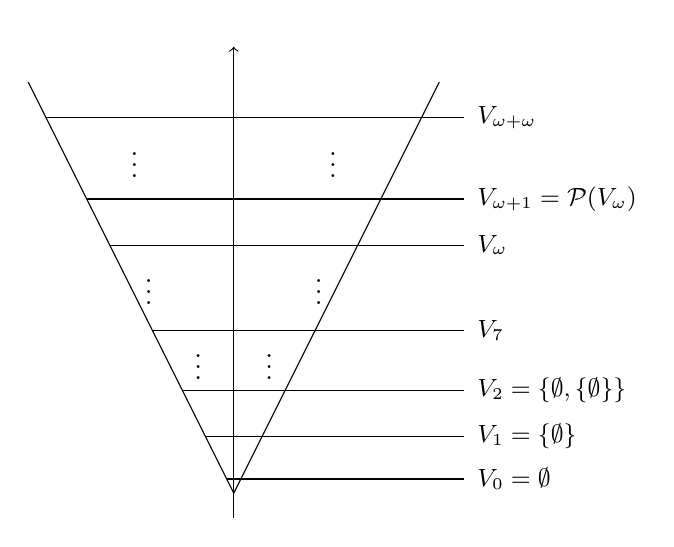
\begin{tikzpicture}[scale=0.9]
    \draw [->] (0, -0.35) -- (0, 6.3) node [above] {$\on$};
    \draw (-2.9, 5.8) -- (0, 0) -- (2.9, 5.8);
    % level lines, each extended by a thin leader out to x = 3.2
    \foreach \h/\lab in {%
      0.2/{$V_0 = \emptyset$},
      0.8/{$V_1 = \{\emptyset\}$},
      1.45/{$V_2 = \{\emptyset, \{\emptyset\}\}$},
      2.3/{$V_7$},
      3.5/{$V_\omega$},
      4.15/{$V_{\omega + 1} = \mathcal{P}(V_\omega)$},
      5.3/{$V_{\omega + \omega}$}} {
      \draw ({-\h/2}, \h) -- ({\h/2}, \h);
      \draw[thin] ({\h/2}, \h) -- (3.25, \h);
      \node[right] at (3.3, \h) {\small \lab};
    }
    \node at (-0.5, 1.9) {$\vdots$};
    \node at (0.5, 1.9) {$\vdots$};
    \node at (-1.2, 2.95) {$\vdots$};
    \node at (1.2, 2.95) {$\vdots$};
    \node at (-1.4, 4.75) {$\vdots$};
    \node at (1.4, 4.75) {$\vdots$};
  \end{tikzpicture}
\end{center}

Every set will turn out to appear somewhere in this cone. Note first that $x \subseteq V_\alpha$ if and only if $x \in V_{\alpha^+}$, straight from the definition.

\begin{lemma}\label{lem:Valphatransitive}
  Each $V_\alpha$ is transitive.
\end{lemma}
\begin{proof}
  Induct on $\alpha$. Certainly $V_0 = \emptyset$ is transitive. If $V_\alpha$ is transitive and $x \in y \in \mathcal{P}(V_\alpha)$, then $y \subseteq V_\alpha$, so $x \in V_\alpha$, so $x \subseteq V_\alpha$ by transitivity, so $x \in \mathcal{P}(V_\alpha)$. Finally a union of transitive sets is transitive, which handles limits.
\end{proof}

\begin{lemma}\label{lem:Valphaincreasing}
  If $\alpha \leq \beta$ then $V_\alpha \subseteq V_\beta$.
\end{lemma}
\begin{proof}
  Fix $\alpha$ and induct on $\beta \geq \alpha$. The case $\beta = \alpha$ is trivial. Given $V_\alpha \subseteq V_\beta$, we have $V_\beta \subseteq \mathcal{P}(V_\beta)$ -- since $x \in V_\beta$ implies $x \subseteq V_\beta$ by Lemma~\ref{lem:Valphatransitive} -- so $V_\alpha \subseteq \mathcal{P}(V_\beta) = V_{\beta^+}$. Limits are immediate from the definition.
\end{proof}

\begin{theorem}[Every Set has a Rank]\label{thm:everysetinV}
  Every set $x$ belongs to some $V_\alpha$.
\end{theorem}
\begin{proof}
  We show $(\forall x)(\exists \alpha)(x \in V_\alpha)$ by $\in$-induction on $x$. So we may assume that each $y \in x$ lies in some $V_\alpha$, and hence that each $y \in x$ has a least $\alpha$ with $y \subseteq V_\alpha$; call it $\rank(y)$, so that $y \in V_{\rank(y)^+}$.

  Let $\alpha = \sup\{\rank(y)^+ \mid y \in x\}$, which is a set by replacement. Then $y \in V_\alpha$ for every $y \in x$ by Lemma~\ref{lem:Valphaincreasing}, so $x \subseteq V_\alpha$ and therefore $x \in V_{\alpha^+}$.
\end{proof}

So $V = \bigcup_{\alpha \in \on} V_\alpha$: the picture above really is the whole universe. This is the sense in which the axiom of foundation succeeds in saying that every set is built out of simpler sets.

\begin{definition}[Rank]
  The \vocab{rank} of a set $x$ is defined by $\in$-recursion by
  $$
\rank(x) = \sup \{\rank(y)^+ \mid y \in x\}.
  $$
\end{definition}

\begin{proposition}
  $\rank(x)$ is the least $\alpha$ with $x \subseteq V_\alpha$, equivalently the least $\alpha$ with $x \in V_{\alpha^+}$.
\end{proposition}
\begin{proof}
  This is precisely what the proof of Theorem~\ref{thm:everysetinV} showed, by $\in$-induction.
\end{proof}

For example $\rank(\emptyset) = 0$, $\rank(n) = n$ for $n \in \omega$, $\rank(\omega) = \omega$, and $\rank(\alpha) = \alpha$ for every ordinal $\alpha$. Note also that $V_\omega$ is precisely the collection of \emph{hereditarily finite} sets -- those which are finite, whose members are finite, and so on -- and it is a model of every axiom of $\ZF$ except infinity.

\begin{example}[Some Ranks]
  We have $\rank(\emptyset) = 0$, and $\rank(\{x\}) = \rank(x)^+$. So $\rank(n) = n$ for $n \in \omega$, and more generally $\rank(\alpha) = \alpha$ for every ordinal $\alpha$: by $\in$-induction, $\rank(\alpha) = \sup\{\rank(\beta)^+ \mid \beta \in \alpha\} = \sup\{\beta^+ \mid \beta < \alpha\} = \alpha$. Also $\rank(\{\omega, \{\omega\}\}) = \omega + 2$.
\end{example}

\begin{example}[$V_\omega$ and $V_{\omega+\omega}$]
  The set $V_\omega$ consists of the \vocab{hereditarily finite} sets: those which are finite, all of whose members are finite, and so on. It is a model of every axiom of $\ZF$ except infinity, so infinity is not a consequence of the others. Similarly $V_{\omega+\omega}$ satisfies every axiom except replacement -- the function-class $n \mapsto V_{\omega + n}$ has image unbounded in $V_{\omega+\omega}$ -- so replacement does not follow from the rest either. Note that $V_{\omega + \omega}$ is a perfectly comfortable place to do most of mathematics: it contains $\N$, $\R$, all the usual function spaces, and so on.
\end{example}

\begin{remark}
  The axiom of foundation is not needed for ordinary mathematics -- one never wants a set with $x \in x$ -- and indeed $\ZF$ without foundation is consistent if $\ZF$ is. What foundation buys us is precisely the picture above: it says that $V$ has no `extra' sets floating outside the cumulative hierarchy. Without it, $\bigcup_\alpha V_\alpha$ would still be a perfectly good model of the other axioms, in which foundation then holds.
\end{remark}

\subsection{The Reflection Principle}

We close this section with a striking consequence of replacement, which says that any finite piece of the theory of $V$ is already visible in some $V_\alpha$.

\begin{theorem}[Reflection Principle]
  Let $p_1, \dots, p_n$ be formulae. Then for every ordinal $\beta$ there is $\alpha > \beta$ such that each $p_i$ holds in $V_\alpha$ (with all parameters taken from $V_\alpha$) if and only if it holds in $V$.
\end{theorem}
\begin{proof}[Proof sketch]
  We may assume the $p_i$ are closed under subformulae. For each subformula of the form $(\exists x) q(x, \vec y)$ define a function-class sending $\vec y$ to the least $\gamma$ such that, if such an $x$ exists at all, one exists in $V_\gamma$; this is legitimate by replacement, since the ordinals are well-ordered. Given $\alpha_0 = \beta$, let $\alpha_{k+1}$ be an ordinal above $\alpha_k$ large enough that $V_{\alpha_{k+1}}$ contains a witness for every existential subformula with parameters in $V_{\alpha_k}$, and set $\alpha = \sup_k \alpha_k$. Then $V_\alpha$ has a witness for each existential subformula whose parameters lie in $V_\alpha$, and an induction on the structure of the formulae shows that each $p_i$ holds in $V_\alpha$ if and only if it holds in $V$.
\end{proof}

One consequence is worth noting: assuming $\ZF$ is consistent, it is not finitely axiomatisable. For suppose $\ZF$ were equivalent to a finite list of sentences $p_1, \dots, p_n$. Applying reflection to these gives an ordinal $\alpha$ with each $p_i$ holding in $V_\alpha$, so $\ZF$ would prove that some \emph{set} is a model of $\ZF$; by the soundness theorem this gives $\ZF \vdash \Con(\ZF)$, contradicting G\"odel's second incompleteness theorem in Section~\ref{sec:incompleteness}.

\section{Cardinals}\label{sec:cardinals}

Ordinals measure the \emph{length} of a well-ordering. Cardinals measure the \emph{size} of a set. We work in $\ZFC$ throughout, and note where choice is used.

\subsection{Cardinality}

We write $x \leftrightarrow y$ to mean $(\exists f)(f \text{ is a bijection from } x \text{ to } y)$. We would like to attach to each set $x$ an object $\card(x)$ such that $\card(x) = \card(y)$ if and only if $x \leftrightarrow y$. The obvious candidate, the collection of all sets bijecting with $x$, is a proper class, so we must be cleverer. In $\ZFC$ there is an easy fix.

\begin{definition}[Cardinality]
  The \vocab{cardinality} of a set $x$, written $\card(x)$, is the least ordinal $\alpha$ with $x \leftrightarrow \alpha$.
\end{definition}

This exists by the well-ordering principle: some well-ordering of $x$ has an order type $\alpha$ with $x \leftrightarrow \alpha$, and then Proposition~\ref{prop:ordinalswo} gives a least one.

\begin{remark}[Scott's Trick]
  In $\ZF$ alone there may be no ordinal bijecting with $x$. Instead define the \vocab{essential rank} of $x$ to be the least $\alpha$ such that some $y$ with $y \leftrightarrow x$ has $\rank(y) = \alpha$, and set
  $$\card(x) = \{y \in V_{\alpha^+} \mid y \leftrightarrow x\},$$
  which is a non-empty set with the required property. This device -- replacing an equivalence class by its members of least rank -- works for any equivalence relation on $V$.
\end{remark}

\begin{definition}[Cardinal]
  A set $m$ is a \vocab{cardinal} if $m = \card(x)$ for some set $x$.
\end{definition}

We use lower case letters $m, n$ for cardinals and the corresponding upper case letters $M, N$ for sets having those cardinalities.

\begin{definition}[Cardinal Inequality]
  For cardinals $m, n$ we write $m \leq n$ if $M$ injects into $N$, and $m < n$ if $m \leq n$ and $m \neq n$.
\end{definition}

This is well-defined (independent of representatives), and it is a partial order: antisymmetry is precisely the Schr\"oder--Bernstein theorem, Corollary~\ref{cor:csb}. In $\ZFC$ it is a total order, since any two sets can be well-ordered and then compared by Proposition~\ref{prop:wotrichotomy}.

\subsection{The Alephs}

Which ordinals are cardinals? Since $\omega \leftrightarrow \omega + 1 \leftrightarrow \omega \cdot 2 \leftrightarrow \omega^2$, most of them are not.

\begin{definition}[Initial Ordinal]
  An ordinal $\alpha$ is \vocab{initial} if no $\beta < \alpha$ has $\beta \leftrightarrow \alpha$; that is, if it is the least ordinal of its cardinality.
\end{definition}

So the cardinals which are ordinals are exactly the initial ordinals. Every finite ordinal is initial, as are $\omega$ and $\gamma(x)$ for any set $x$ (by minimality in Hartogs' lemma).

\begin{definition}[The Omegas]
  Define $\omega_\alpha$ for $\alpha \in \on$ by transfinite recursion:
  \begin{align*}
    \omega_0 &= \omega, \\
    \omega_{\alpha^+}&= \gamma(\omega_\alpha), \\
    \omega_{\lambda} &= \sup\{\omega_\alpha\mid \alpha < \lambda\} \quad \text{for } \lambda \text{ a non-zero limit.}
  \end{align*}
\end{definition}

\begin{proposition}
  Each $\omega_\alpha$ is initial, and every infinite initial ordinal is some $\omega_\alpha$.
\end{proposition}
\begin{proof}
  That each $\omega_\alpha$ is initial follows by induction: $\gamma$ of an ordinal is initial, and a supremum of initial ordinals is initial (if $\beta < \omega_\lambda$ bijected with $\omega_\lambda$ then $\beta < \omega_\alpha$ for some $\alpha < \lambda$, and $\omega_\lambda$ would inject into $\omega_\alpha$).

  Conversely let $\delta \geq \omega$ be initial. By induction $\omega_\alpha \geq \alpha$ for every $\alpha$, so the $\omega_\alpha$ are unbounded and there is a least $\epsilon$ with $\delta < \omega_\epsilon$. This $\epsilon$ is not a limit (else $\delta < \omega_\alpha$ for some $\alpha < \epsilon$) and not zero (as $\delta \geq \omega = \omega_0$), so $\epsilon = \alpha^+$ and $\omega_\alpha \leq \delta < \omega_{\alpha^+} = \gamma(\omega_\alpha)$. Then $\delta$ injects into $\omega_\alpha$, so being initial forces $\delta = \omega_\alpha$.
\end{proof}

\begin{definition}[Aleph]
  We write $\aleph_\alpha = \card(\omega_\alpha)$.
\end{definition}

We use a separate symbol because $\card$ may be defined by Scott's trick rather than as an ordinal. From the proposition, the $\aleph_\alpha$ are precisely the cardinalities of the infinite sets -- or, in $\ZF$ without choice, of the infinite \emph{well-orderable} sets.

\subsection{Cardinal Arithmetic}

\begin{definition}[Cardinal Arithmetic]
  For cardinals $m, n$ we define
  $$m + n = \card(M \sqcup N), \qquad mn = \card(M \times N), \qquad m^n = \card(M^N),$$
  where $M^N = \{f \mid f \text{ is a function } N \to M\}$.
\end{definition}

These do not depend on the choice of representatives. Unlike ordinal arithmetic, cardinal addition and multiplication are commutative and associative, and satisfy the usual laws such as $(m^n)^p = m^{np}$ -- the last because a function $P \to (N \to M)$ is the same thing as a function $N \times P \to M$. Note that the notation clashes with ordinal arithmetic: $2^\omega = \omega$ as ordinals, but $2^{\aleph_0} > \aleph_0$ as cardinals. Which is meant is always determined by whether the symbols are ordinals or cardinals.

\begin{example}
  $\R \leftrightarrow \mathcal{P}(\omega) \leftrightarrow \{0,1\}^\omega$, so $\card(\R) = \card(\mathcal{P}(\omega)) = 2^{\aleph_0}$.
\end{example}

\begin{example}[How Many Sequences of Reals?]
  A real sequence is a function $\omega \to \R$, so the answer is
  $$\card(\R^\omega) = (2^{\aleph_0})^{\aleph_0} = 2^{\aleph_0 \cdot \aleph_0} = 2^{\aleph_0} = \card(\R),$$
  using $\aleph_0 \aleph_0 = \aleph_0$, which holds since $\omega \times \omega \leftrightarrow \omega$.
\end{example}

\begin{theorem}[Cantor]
  For every cardinal $m$ we have $m < 2^m$.
\end{theorem}
\begin{proof}
  Certainly $m \leq 2^m$, as $x \mapsto \{x\}$ injects $M$ into $\mathcal{P}(M)$. Suppose $f: M \to \mathcal{P}(M)$ were a bijection, and let $A = \{x \in M \mid x \notin f(x)\}$. Then $A = f(a)$ for some $a \in M$, and now $a \in A$ if and only if $a \notin f(a) = A$, which is absurd.
\end{proof}

\begin{example}[More Cardinal Computations]~
  \begin{enumerate}[label=(\roman*)]
    \item There are $2^{\aleph_0}$ continuous functions $\R \to \R$. Each is determined by its restriction to $\Q$, so there are at most $\card(\R^\Q) = (2^{\aleph_0})^{\aleph_0} = 2^{\aleph_0}$ of them, and at least that many since the constants are continuous.
    \item There are $2^{2^{\aleph_0}}$ functions $\R \to \R$ altogether, namely $\card(\R^\R) = (2^{\aleph_0})^{2^{\aleph_0}} = 2^{\aleph_0 \cdot 2^{\aleph_0}} = 2^{2^{\aleph_0}}$. So `almost no' function is continuous.
    \item The set of finite sequences from an infinite set $X$ has the same cardinality as $X$, since $\sum_{n < \omega} m^n = \aleph_0 \cdot m = m$ using Theorem~\ref{thm:alephsquared}. In particular there are only countably many formulae in a countable language, which is the fact we used repeatedly in Sections~\ref{sec:predicate} and~\ref{sec:incompleteness}.
  \end{enumerate}
\end{example}

That last fact generalises completely, and it makes cardinal addition and multiplication of infinite cardinals utterly uninteresting.

\begin{theorem}\label{thm:alephsquared}
  For every ordinal $\alpha$ we have $\aleph_\alpha \aleph_\alpha = \aleph_\alpha$.
\end{theorem}
\begin{proof}
  We induct on $\alpha$. Define a well-ordering of $\omega_\alpha \times \omega_\alpha$ by `going up in squares': set $(x, y) < (z, w)$ if
  \begin{itemize}
    \item $\max(x, y) < \max(z, w)$; or
    \item $\max(x,y) = \max(z,w) = \beta$, and one of: $y < \beta$ and $z < \beta$; or $x = z = \beta$ and $y < w$; or $y = w = \beta$ and $x < z$.
  \end{itemize}
  In words, we enumerate the pairs by sweeping out successively larger square blocks, and within the $\beta$-th block we go up the left edge and then along the top.

  Given $\delta \in \omega_\alpha \times \omega_\alpha$ we have $\delta \in \beta \times \beta$ for some $\beta < \omega_\alpha$, as $\omega_\alpha$ is a limit. By the induction hypothesis $\beta \times \beta \leftrightarrow \beta$ (or $\beta$ is finite), so the initial segment $I_\delta$ is contained in $\beta \times \beta$ and hence
  $$\card(I_\delta) \leq \card(\beta \times \beta) = \card(\beta) < \card(\omega_\alpha).$$
  So every proper initial segment of our well-ordering is smaller than $\omega_\alpha$, meaning its order type is at most $\omega_\alpha$. Hence $\omega_\alpha \times \omega_\alpha$ injects into $\omega_\alpha$, and the reverse injection is obvious, so they biject by Schr\"oder--Bernstein.
\end{proof}

\begin{corollary}
  For ordinals $\alpha \leq \beta$ we have $\aleph_\alpha + \aleph_\beta = \aleph_\alpha \aleph_\beta = \aleph_\beta$.
\end{corollary}
\begin{proof}
  $\aleph_\beta \leq \aleph_\alpha+\aleph_\beta \leq 2 \aleph_\beta \leq \aleph_\alpha \aleph_\beta \leq \aleph_\beta^2=\aleph_\beta$.
\end{proof}

So, for instance, $X \sqcup X \leftrightarrow X$ and $X \times X \leftrightarrow X$ for every infinite set $X$ -- results which in $\ZF$ alone are not provable.

Cardinal \emph{exponentiation}, by contrast, is genuinely hard. We know $m < 2^m$ for all $m$ by Cantor's diagonal argument, so $\aleph_0 < 2^{\aleph_0}$, and $\aleph_1 \leq 2^{\aleph_0}$ since $2^{\aleph_0}$ is the cardinality of an uncountable well-orderable set. Whether equality holds -- the \vocab{Continuum Hypothesis} -- is independent of $\ZFC$: G\"odel showed it is consistent with $\ZFC$, and Cohen showed its negation is too. $\ZFC$ does not even decide whether $2^{\aleph_0} < 2^{\aleph_1}$.

It is convenient to name the cardinals obtained by iterating the power set.

\begin{definition}[Beth Numbers]
  Define $\beth_0 = \aleph_0$, $\beth_{\alpha^+} = 2^{\beth_\alpha}$, and $\beth_\lambda = \sup\{\beth_\alpha \mid \alpha < \lambda\}$ for a non-zero limit $\lambda$.
\end{definition}

So $\beth_1 = 2^{\aleph_0} = \card(\R)$, and by Cantor's theorem $\beth_\alpha \geq \aleph_\alpha$ for all $\alpha$. The \vocab{generalised continuum hypothesis} is the assertion that $\beth_\alpha = \aleph_\alpha$ for every $\alpha$, that is, that $2^{\aleph_\alpha} = \aleph_{\alpha^+}$; like the continuum hypothesis it is independent of $\ZFC$. Note that $\beth_\omega$ is a cardinal with $\beth_\omega = \sup_n \beth_n$, so it is a limit of cardinals reached from below by a sequence of length $\omega$ -- which brings us to our last topic.

\subsection{Cofinality}

There is, however, one genuine constraint on cardinal exponentiation, and it comes from the following notion.

\begin{definition}[Cofinality]
  The \vocab{cofinality} $\cf(\alpha)$ of a limit ordinal $\alpha$ is the least order type of a subset of $\alpha$ which is unbounded in $\alpha$. An infinite cardinal $\omega_\alpha$ is \vocab{regular} if $\cf(\omega_\alpha) = \omega_\alpha$, and \vocab{singular} otherwise.
\end{definition}

\begin{example}
  $\cf(\omega) = \omega$, so $\omega$ is regular. Also $\cf(\omega_1) = \omega_1$: we saw in Section~\ref{sec:ordarith} that every countable subset of $\omega_1$ is bounded, so no subset of order type less than $\omega_1$ is unbounded. On the other hand $\cf(\omega \cdot 2) = \omega$, and $\cf(\aleph_\omega) = \omega$ since $\aleph_\omega = \sup\{\aleph_n \mid n < \omega\}$, so $\aleph_\omega$ is singular.
\end{example}

The argument for $\omega_1$ generalises: for any $\alpha$, the cardinal $\aleph_{\alpha^+}$ is regular, since a union of $\aleph_\alpha$ sets each of size $\aleph_\alpha$ has size $\aleph_\alpha$ by Theorem~\ref{thm:alephsquared}. So successor cardinals are regular (in $\ZFC$), and only limit cardinals such as $\aleph_\omega$ can be singular.

\begin{proposition}
  For any limit ordinal $\alpha$, the ordinal $\cf(\alpha)$ is a regular cardinal.
\end{proposition}
\begin{proof}
  Let $\gamma = \cf(\alpha)$ and let $S \subseteq \alpha$ be unbounded of order type $\gamma$. If $T \subseteq \gamma$ were unbounded in $\gamma$ of order type $\delta < \gamma$, then the corresponding subset of $S$ would be unbounded in $\alpha$ and have order type $\delta$, contradicting minimality of $\gamma$. So $\cf(\gamma) = \gamma$. In particular $\gamma$ is initial, since a bijection with a smaller ordinal would give an unbounded subset of order type less than $\gamma$.
\end{proof}

Cofinality bounds exponentiation from below.

\begin{theorem}[K\"onig]
  For every infinite cardinal $m$ we have $\cf(2^m) > m$.
\end{theorem}
\begin{proof}[Proof sketch]
  Suppose $2^m = \sup\{n_i \mid i \in I\}$ with $|I| \leq m$ and each $n_i < 2^m$. Writing $2^m$ as the set of functions $M \to \{0,1\}$ and splitting it into $|I|$ pieces of size $n_i$, a diagonal argument produces a function differing from everything in every piece, which is a contradiction.
\end{proof}

In particular $2^{\aleph_0} \neq \aleph_\omega$, since $\cf(\aleph_\omega) = \omega$. So although $\ZFC$ is nearly silent about $2^{\aleph_0}$, it is not completely silent.

\section{Incompleteness}\label{sec:incompleteness}

We finish by returning to Peano arithmetic. Our aim is to show that $\PA$ is \emph{incomplete}: there is a sentence $p$ with $\PA \not\vdash p$ and $\PA \not\vdash \lnot p$. Since one of $p$, $\lnot p$ must hold in $\N$, this produces a sentence which is true (in $\N$) but unprovable.

Note that this is not in tension with the completeness theorem, which says that $\PA \vdash p$ whenever $p$ holds in every model of $\PA$. What it will show is that the non-standard models of Section~\ref{sec:predicate} cannot be legislated away.

The strategy is beautiful and simple to state: we find a sentence $p$ which asserts `$p$ is not provable in $\PA$'. Then $p$ is true if and only if $p$ is unprovable. If $p$ were false, it would be provable and hence true by soundness, a contradiction; so $p$ is true, and therefore unprovable. All the work is in making a sentence of arithmetic talk about sentences of arithmetic.

Throughout, `true' means true in $\N$ and `provable' means provable in $\PA$.

\subsection{Definability}

\begin{definition}[Definable]
  A subset $S \subseteq \N$ is \vocab{definable} if there is a formula $p$ with one free variable $x$ such that for all $m \in \N$, we have $m \in S$ if and only if $p[m/x]$ is true. A function $f: \N \to \N$ is \vocab{definable} if there is a formula $p$ with free variables $x, y$ such that $f(m) = n$ if and only if $p[m/x, n/y]$ is true.
\end{definition}

\begin{example}
  The set of squares is definable by $(\exists y)(y \cdot y = x)$. The set of primes is definable by
  $$x \neq 1 \land (\forall y)(\forall z)(y \cdot z = x \Rightarrow (y = 1 \lor z = 1)).$$
  The function $x \mapsto \lfloor x/2 \rfloor$ is definable by $(x = 2y) \lor (x = 2y + 1)$. The set of powers of $2$ is definable by `every prime dividing $x$ equals $2$'.
\end{example}

Since there are only countably many formulae, only countably many subsets of $\N$ are definable. The fact we need, which we shall not prove, is a converse of sorts: \emph{every function or set given by an algorithm is definable in $\PA$}.

The precise statement runs through primitive recursion.

\begin{definition}[Primitive Recursive]
  The \vocab{primitive recursive} functions $\N^k \to \N$ are those obtained from
  \begin{enumerate}[label=(\roman*)]
    \item the constant $0$, the successor function $s$, and the projections $(x_1, \dots, x_k) \mapsto x_i$,
  \end{enumerate}
  by finitely many applications of
  \begin{enumerate}[label=(\roman*), start=2]
    \item \emph{composition}: from $g$ and $h_1, \dots, h_m$ form $\vec x \mapsto g(h_1(\vec x), \dots, h_m(\vec x))$;
    \item \emph{primitive recursion}: from $g$ and $h$ form the function $f$ satisfying $f(\vec x, 0) = g(\vec x)$ and $f(\vec x, n^+) = h(\vec x, n, f(\vec x, n))$.
  \end{enumerate}
\end{definition}

Addition, multiplication, exponentiation, factorials, `the $n$th prime', bounded sums and products, and the characteristic functions of `$x$ divides $y$' and `$x$ is prime' are all primitive recursive, by writing down the recursions. One then shows that every primitive recursive function is definable in $\PA$, essentially by coding the finite sequence of intermediate values with the prime-power trick of the next section. Every function we need below is primitive recursive, so we may take definability for granted.

\subsection{Coding}

The language of $\PA$ has the symbols
$$0, \; s, \; +, \; \cdot, \; =, \; \bot, \; \Rightarrow, \; (, \; ), \; \forall, \; x, \; {}',$$
where variables are $x, x', x'', \dots$. Assign to each symbol a number, say $v(0) = 1$, $v(s) = 2$, \dots, $v(') = 12$. Then encode a formula $p$ with symbols $\sigma_1 \sigma_2 \cdots \sigma_n$ by
$$c(p) = 2^{v(\sigma_1)} \, 3^{v(\sigma_2)} \, 5^{v(\sigma_3)} \cdots (n\text{th prime})^{v(\sigma_n)}.$$

\begin{center}
  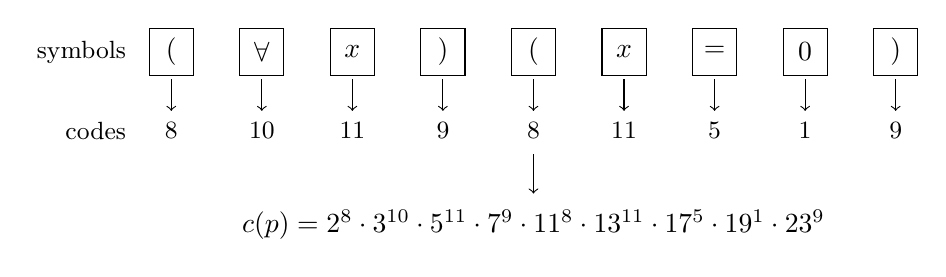
\begin{tikzpicture}[scale=1]
    \foreach \i/\s in {0/{$($}, 1/{$\forall$}, 2/{$x$}, 3/{$)$}, 4/{$($}, 5/{$x$}, 6/{$=$}, 7/{$0$}, 8/{$)$}} {
      \draw (\i*1.15 - 0.28, 1.05) rectangle (\i*1.15 + 0.28, 1.65);
      \node at (\i*1.15, 1.35) {\s};
    }
    \foreach \i/\n in {0/8, 1/10, 2/11, 3/9, 4/8, 5/11, 6/5, 7/1, 8/9} {
      \node at (\i*1.15, 0.35) {\small $\n$};
      \draw[->] (\i*1.15, 1.0) -- (\i*1.15, 0.6);
    }
    \node[left] at (-0.45, 1.35) {\small symbols};
    \node[left] at (-0.45, 0.35) {\small codes};
    \draw[->] (4.6, 0.05) -- (4.6, -0.45);
    \node at (4.6, -0.85) {$c(p) = 2^{8} \cdot 3^{10} \cdot 5^{11} \cdot 7^{9} \cdot 11^{8} \cdot 13^{11} \cdot 17^{5} \cdot 19^{1} \cdot 23^{9}$};
  \end{tikzpicture}
\end{center}

By unique factorisation, we can recover $p$ from $c(p)$. Not every number codes a formula, and we write $S_n$ for the formula coded by $n$, taking $S_n = \bot$ if $n$ codes nothing.

The point of all this is that the syntactic notions we care about become arithmetical statements about codes, each of which is decided by an algorithm and hence is definable:
\begin{enumerate}[label=(\roman*)]
  \item `$n$ codes a formula';
  \item `$n$ codes a formula with exactly one free variable';
  \item `$l, m, n$ code formulae and $S_n$ follows from $S_l, S_m$ by modus ponens', and similarly for generalisation;
  \item `$n$ codes a logical axiom or an axiom of $\PA$'.
\end{enumerate}
Sequences of formulae are coded the same way, by
$$s(p_1, \dots, p_n) = 2^{c(p_1)} 3^{c(p_2)} \cdots (n\text{th prime})^{c(p_n)},$$
and then `$n$ codes a proof' and `$n$ codes a proof of $S_m$' are definable too. Let $\theta(m, n)$ be a formula defining `$n$ codes a proof of $S_m$'. Then
$$\phi(m) = (\exists n)\,\theta(m, n)$$
defines `$S_m$ is provable'.

\subsection{G\"odel's Incompleteness Theorems}

Now for the clever bit. Consider the statement
$$\chi(m) = \text{`$m$ codes a formula $S_m$ with one free variable, and $S_m[m/x]$ is unprovable'}.$$
This is again decided by an algorithm applied to the definable ingredients above, so it is definable: there is a formula $p$ with one free variable such that $\chi(m)$ holds if and only if $p[m/x]$ is true.

Let $N = c(p)$, so $S_N = p$. Then $p[N/x]$ says precisely that $N$ codes a formula with one free variable whose substitution instance at $N$ is unprovable. But that substitution instance is $S_N[N/x] = p[N/x]$ itself. So
$$p[N/x] \text{ asserts that } p[N/x] \text{ is unprovable},$$
which is exactly the self-referential sentence we wanted.

\begin{theorem}[G\"odel's First Incompleteness Theorem]
  $\PA$ is incomplete: there is a sentence which is true in $\N$ but not provable in $\PA$.
\end{theorem}
\begin{proof}
  Let $q$ be the sentence $p[N/x]$ constructed above, so that $q$ is true if and only if $q$ is unprovable. If $q$ is false then $q$ is provable, hence true by soundness -- a contradiction. So $q$ is true, and therefore unprovable. As $q$ is true, $\lnot q$ is false and so also unprovable, again by soundness.
\end{proof}

Note that nothing in this argument is special to $\PA$: it applies to any consistent theory strong enough to code its own syntax, and to which we have added any true sentences we like. So we cannot repair $\PA$ by adding axioms, provided that we can still recognise the axioms algorithmically.

\begin{theorem}[G\"odel's Second Incompleteness Theorem]
  $\PA \not\vdash \Con(\PA)$, where $\Con(\PA)$ is the sentence $(\forall n)(n \text{ does not code a proof of } \bot)$.
\end{theorem}
\begin{proof}[Proof sketch]
  Examining the proof above, the only external ingredient was soundness, which we used via the existence of a model of $\PA$ -- and any model would do. So the argument formalises inside $\PA$ itself, to give
  $$\PA \cup \{\Con(\PA)\} \vdash q.$$
  If $\PA \vdash \Con(\PA)$ we would then have $\PA \vdash q$, contradicting the first incompleteness theorem.
\end{proof}

Finally, let $T$ be the set of all sentences true in $\N$. This is a complete theory extending $\PA$, so the argument above must break down for it -- and the only step which can fail is the definability of the syntactic notions. So we obtain the following.

\begin{theorem}[Undecidability of Truth]
  There is no algorithm to decide whether a sentence of arithmetic is true in $\N$. Equivalently, the set $\{c(p) \mid p \in T\}$ is not definable.
\end{theorem}

\begin{remark}[The Entscheidungsproblem]
  In Section~\ref{sec:predicate} we noted that there is no analogue of the decidability theorem for predicate logic. The methods of this section are what settle the matter: the set of theorems of predicate logic in a language with a single binary relation symbol is not decidable, since one may code arithmetic into it. What \emph{is} true is that the theorems are recursively enumerable -- by the completeness theorem we may simply enumerate all proofs -- so validity is semi-decidable. Truth in $\N$, by the theorem above, is not even that.
\end{remark}

The same phenomena occur higher up. $\ZFC$ proves that $\PA$ has a model, namely $\omega$, so $\ZFC \vdash \Con(\PA)$ -- which by the second incompleteness theorem shows that $\ZFC$ is strictly stronger than $\PA$. But $\ZFC$ can code its own syntax just as well as $\PA$ can, so if $\ZFC$ is consistent then $\ZFC$ is incomplete, and $\ZFC \not\vdash \Con(\ZFC)$. There is no escape by moving to a stronger theory: any consistent, recognisable set of axioms strong enough to do arithmetic will leave some true statement unproved.

